%  Gustavo Voltani von Atzingen 
%   Iniciado em: 25/05/2014
%  
%  Base para a qualificação e defesa de Doutorado
%
%  Referencias de layout utilizadas: 
%   - https://code.google.com/p/mestre-em-latex/
%   - 

\documentclass[a4paper,12pt, oneside]{report}
%%% Pacotes utilizados %%%

%% Codificação e formatação básica do LaTeX
% Suporte para português (hifenação e caracteres especiais)
\usepackage[english,brazilian]{babel}

% Codificação do arquivo
\usepackage[utf8]{inputenc}

% Opções de fixar a imagem após um parágrafo /figure{fsdsd}[H]
\usepackage{float}

% Mapear caracteres especiais no PDF
\usepackage{cmap}

% Codificação da fonte
\usepackage[T1]{fontenc}
% Usa a lmodern por padrão (caso cm-super não esteja instalada).
\usepackage{lmodern}

%% Microtipografia
% Utiliza recursos como espaçamento entre letras e entre linhas
\usepackage{microtype}
% Habilita protrusão e expansão, ignorando
% compatibilidade (ver documentação do pacote)
\microtypesetup{activate={true,nocompatibility}}
% factor=1100 aumenta a protrusão (default 1000)
% stretch=10 diminui o valor máximo de expansão (default 20)
% shrink=10 diminui o valor máximo de encolhimento (default 20)
\microtypesetup{factor=1100, stretch=10, shrink=10}
% Tracking, espaçamento entre palavras, kerning
\microtypesetup{tracking=true, spacing=true, kerning=true}
% Remover tracking para Small Caps
\SetTracking{encoding={T1}, shape=sc}{0}
% Remove ligaduras para o 'f'. Se necessário, adicionar letras
% separadas por vírgulas
\DisableLigatures[f]{encoding={T1}}
% Documento em versão "final", suporte para outros idiomas
\microtypesetup{final, babel}

% Essencial para colocar funções e outros símbolos matemáticos
\usepackage{amsmath,amssymb,amsfonts,textcomp}

%% Layout
% Customização do layout da página, margens espelhadas
\usepackage[]{geometry}
% Aumenta as margens internas para espiral
%\geometry{centering}
% Só pra ajustar o layout
\setlength{\marginparwidth}{90pt}
%\usepackage{layout}

% Para definir espaçamento entre as linhas
\usepackage{setspace}

% Espaçamento do texto para o frame
\setlength{\fboxsep}{1em}

% Faz com que as margens tenham o mesmo tamanho horizontalmente
%\geometry{hcentering}

%% Elementos Gráficos
% Para incluir figuras (pacote extendido)
\usepackage[]{graphicx}

%% Suporte a cores
\usepackage{color}
% Os argumentos declaram nomes novos, como Cyan e Crimson
% (ver documentação do pacote).
\usepackage[usenames,dvipsnames,svgnames]{xcolor}

\usepackage{chngcntr}
\counterwithout{figure}{chapter}
% Criar figura dividida em subfiguras
\usepackage{subfig}
\captionsetup[subfigure]{style=default, margin=0pt, parskip=0pt, hangindent=0pt, indention=0pt, singlelinecheck=true, labelformat=parens, labelsep=space}

% Caso queira guardar as figuras em uma pasta separada
% (descomente e) defina o caminho para o diretório:
\graphicspath{{./Figuras/}}

% Customizar as legendas de figuras e tabelas
\usepackage{caption}

% Criar ambientes com 2 ou mais colunas
\usepackage{multicol}

% Ative o comando abaixo se quiser colocar figuras de fundo (e.g., capa)
%\usepackage{wallpaper}
% Exemplo para inserir a figura na capa está no arquivo pre.tex (linha 7)
% Ajuste da posição da figura no eixo Y
%\addtolength{\wpYoffset}{-140pt}
% Ajuste da posição da figura no eixo X
%\addtolength{\wpXoffset}{36pt}

%% Tabelas
% Elementos extras para formatação de tabelas
\usepackage{array}

% Tabelas com qualidade de publicação
\usepackage{booktabs}

% Para criar tabelas maiores que uma página
\usepackage{longtable}

% adicionar tabelas e figuras como landscape
\usepackage{lscape}

%% Lista de Abreviações
% Cria lista de abreviações
%\usepackage[notintoc,portuguese]{nomencl}
%\makenomenclature

%% Notas de rodapé
% Lidar com notas de rodapé em diversas situações
\usepackage{footnote}

% Notas criadas nas tabelas ficam no fim das tabelas
\makesavenoteenv{tabular}

% Conta o número de páginas
\usepackage{lastpage}

%% Referências bibliográficas e afins
% Formatar as citações no texto e a lista de referências
\usepackage{natbib}
%\usepackage{abntex2cite}

% Adicionar bibliografia, índice e conteúdo na Tabela de conteúdo
% Não inclui lista de tabelas e figuras no índice
\usepackage[nottoc,notlof,notlot]{tocbibind}

%% Pontuação e unidades
% Posicionar inteligentemente a vírgula como separador decimal
\usepackage{icomma}

% Formatar as unidades com as distâncias corretas
\usepackage[tight]{units}

% Pacotes e alterações nos capítulos
\usepackage[Bjornstrup]{fncychap}  %Options: Sonny, Lenny, Glenn, Conny, Rejne, Bjarne, %Bjornstrup

% diagramas - Gustavo
% Insere a biblioteca e coloca as propriedades dos diagramas
\usepackage{tikz}
\usetikzlibrary{shapes,shadows,arrows}
\tikzstyle{decision} = [diamond,draw,fill=blue!50]
%\tikzstyle{line} = [draw,-latex']
\tikzstyle{line} = [line width=0.06cm, ->]
\tikzstyle{elli} = [draw, ellipse, fill=red!50, text width=10em, text centered, minimum height=12mm, node distance=5em]
\tikzstyle{block} = [draw,rectangle, fill=blue!50, text width=10em, text centered, minimum height=12mm, node distance=5em]


\usepackage{lipsum} % filler text
\usepackage{etoolbox}
\makeatletter
\patchcmd{\@makechapterhead}{\vspace*{50\p@}}{\vspace*{-20\p@}}{}{}
\patchcmd{\@makeschapterhead}{\vspace*{50\p@}}{\vspace*{0\p@}}{}{}
\patchcmd{\DOTI}{\vskip 40\p@}{\vskip 50\p@}{}{}
\patchcmd{\DOTIS}{\vskip 40\p@}{\vskip 0\p@}{}{}
\makeatother

%% Cabeçalho e rodapé
% Controlar os cabeçalhos e rodapés
\usepackage{fancyhdr}
% Usar os estilos do pacote fancyhdr
\pagestyle{fancy}
\fancyhf{}
\fancyfoot{}
\rhead{\thepage}
\renewcommand{\headrulewidth}{0pt}
% Omitir linha de separação entre rodapé e conteúdo
\renewcommand{\footrulewidth}{0pt}
% Altura do cabeçalho
\headheight 13.6pt

% Dados do projeto
\newcommand{\nomedoaluno}{Gustavo Voltani von Atzingen}
\newcommand{\titulo}{Simulação, controle e automação de um forno tipo túnel utilizando tecnologia embarcada}
\newcommand{\nomeorientador}{Ernane Jose Xavier Costa}

\newcommand{\mychapter}[2]{
    \setcounter{chapter}{#1}
    \setcounter{section}{0}
    \chapter*{#2}
    \addcontentsline{toc}{chapter}{#2}
}


%% Links dinâmicos
% Suporte para hipertexto, links para referências e figuras
\usepackage{hyperref}
% Configurações dos links e metatags do PDF a ser gerado
\hypersetup{colorlinks=true, linkcolor=black, citecolor=black, filecolor=blue, pagecolor=black, urlcolor=balck,
            pdfauthor={\nomedoaluno},
            pdftitle={\titulo},
            pdfsubject={Assunto do Projeto},
            pdfkeywords={palavra-chave, palavra-chave, palavra-chave},
            pdfproducer={LaTeX},
            pdfcreator={pdfTeX}}

% Para adicionar linhas de código no apendice:
\usepackage{listings}
\usepackage{color}

\definecolor{dkgreen}{rgb}{0,0.6,0}
\definecolor{gray}{rgb}{0.5,0.5,0.5}
\definecolor{mauve}{rgb}{0.58,0,0.82}

\lstset{frame=tb,
  language=Java,
  aboveskip=3mm,
  belowskip=3mm,
  showstringspaces=false,
  columns=flexible,
  basicstyle={\small\ttfamily},
  numbers=none,
  numberstyle=\tiny\color{gray},
  keywordstyle=\color{blue},
  commentstyle=\color{dkgreen},
  stringstyle=\color{mauve},
  breaklines=true,
  breakatwhitespace=true
  tabsize=3
}






    % pacote com as informações de configuração retiradas de: mester-em-latex

\begin{document}

    \pagestyle{plain}
    %\pagestyle{fancyplain}
    %\pagenumbering{roman}
    % Parte Pré-Texto
    % Limpa cabeçalhos.
% (solução para lidar com a númeração das páginas pré-textuais).
\pagestyle{empty}

%% Capa
\begin{titlepage}

% Se quiser uma figura de fundo na capa ative o pacote wallpaper
% e descomente a linha abaixo.
% \ThisCenterWallPaper{0.8}{nomedafigura}

\begin{center}
{\LARGE \nomedoaluno}
\par
\vspace{200pt}
{\Huge \titulo}
\par
\vfill
\textbf{{\large Pirassununga, SP}\\
{\large \the\year}}
\end{center}
\end{titlepage}

% Faz com que a página seguinte sempre seja ímpar (insere pg em branco)
%\cleardoublepage

% Numeração em elementos pré-textuais é opcional (ativada por padrão).
% Para desativá-la comente a linha abaixo.
%\pagestyle{fancy}

% Números das páginas em algarismos romanos
%\pagenumbering{roman}

%% Página de Rosto

% Numeração não deve aparecer na página de rosto.
\thispagestyle{empty}

\begin{center}
{\LARGE \nomedoaluno}
\par
\vspace{200pt}
{\Huge \titulo}
\end{center}
\par
\vspace{90pt}
\hspace*{175pt}\parbox{7.6cm}{{\large Qualificação apresentada à Faculdade de Zootecnia e Engenharia de Alimentos da Universidade de São Paulo, como parte dos requisitos para a obtenção de Título de Doutor em Ciências, na Área de Engenharia de Alimentos.}}

\par
\vspace{1em}
\hspace*{175pt}\parbox{7.6cm}{{\large Orientador: Ernane José Xavier Costa}}

\par
\vfill
\begin{center}
\textbf{{\large Pirassununga, SP}\\
{\large \the\year}}
\end{center}

\newpage

% Ficha Catalográfica
%\hspace{8em}\fbox{\begin{minipage}{10cm}
%Atzingen, Gustavo Voltani von.

%\hspace{2em}\titulo

%\hspace{2em}\pageref{LastPage} páginas

%\hspace{2em}Qualificação apresentada a Faculdade de Zootecnia e Engenharia de Alimentos da Universidade de São Paulo, como %parte dos requisitos para a obtenção de Título de Doutor em Ciências, na Área de Engenharia de Alimentos.

%Area de Concentração: Ciências da Engenharia de Alimentos

%Orientador: Ernane José Xavier Costa

%\begin{enumerate}
%\item Diferenças Finitas
%\item CFD
%\item Raspberry Pi
%\item Arduino
%\end{enumerate}


%\end{minipage}}
%\vspace{2em}

%\newpage
%\pagestyle{fancyplain}
% Desabilitar protrusão para listas e índice
%\microtypesetup{protrusion=false}
   % Capa, contra-capa e folha de rosto
    \doublespacing
    %% Agradecimentos
\newpage

\mychapter{0}{Agradecimentos}\label{agradecimentos}

% Espaçamento duplo
\doublespacing

Agradeço ao meu orientador, ao meu co-orientador, aos meus colaboradores, aos técnicos, à seção administrativa, à fundação que liberou verba para minhas pesquisas, aos meus amigos, à minha família e ao meu grande amor.
    \newpage

\mychapter{0}{Resumo}\label{resumo}
Atzingen, G. V. v. \textbf{Simulação, controle e automação de um forno tipo túnel utilizando tecnologia embarcada.} \pageref{LastPage} f. Qualificação (Doutorado) - Faculdade de Zootecnia e Engenharia de Alimentos, 2014.

\noindent
\\Baseado na grande evolução dos dispositivos eletrônicos nos últimos 35 anos e dos novos hardwares de baixo custo e alto poder computacional, esta tese tem como objetivo apresentar um software e hardware de controle e simulação em tempo real utilizando um sistema embarcado de hardware livre de baixo custo que garanta a qualidade na produção de alimentos em fornos tipo túnel. Para isto, modelagem matemática e simulação do perfil de temperatura dentro do forno foram realizadas para que o sistema de controle possa ter informação da temperatura no alimento em tempo real, contando apenas com os sensores fixos no forno. A informação desta simulação alimenta o controle PID, garantindo que o perfil de temperatura desejado para o aquecimento/cozimento do alimento seja obedecido, melhorando a qualidade do produto final.

\par
\vspace{1em}
\noindent\textbf{Palavras-chave:} Diferenças Finitas, CFD, Raspberry Pi, Arduino
    \newpage

\mychapter{0}{Abstract}\label{abstract}
Atzingen, G. V. v. \textbf{Simulation, control and automation of a conveyor belt tunel oven with embedded technology.} \pageref{LastPage} f. PhD qualify - Faculdade de Zootecnia e Engenharia de Alimentos, 2014.

\noindent
\\Based on the big evolution of the electronic devices in the las 35 years and in the recent new hardwares of low cost computational power, this thesis has the goal of presenting a software and hardware for real time simulation and control of conveyor belt tunnel oven using low cost embedded hardware to ensure the production quality. For this purpose, mathematical modeling and simulation of the temperature profile inside the oven was realized in order to supply the control system with the temperature on the food in real time, using only the fixed sensors of the oven. This simulation information is passed to the PID control, ensuring that the desired temperature profile for the heating of the food is accomplished, improving the quality of the final product.

\par
\vspace{1em}
\noindent\textbf{Key-words:} Finite Diference, CFD, Raspberry Pi, Arduino

    \cleardoublepage % Processo para inserir a lista de figuras no sumário
    \addcontentsline{toc}{chapter}{\listfigurename}
    \listoffigures
    
    \cleardoublepage % Processo para inserir a lista de tabelas no sumário
    \addcontentsline{toc}{chapter}{Lista de Tabelas}    
    \listoftables    % Lista de tabelas
    
    \microtypesetup{protrusion=true}  % Re-habilita protrusão novamente
    \newpage

\mychapter{0}{Siglas}\label{siglas}


\begin{itemize}
  \item IBGE - Instituto Brasileiro de Geografia e Estatística
  \item PIB - Produto Interno Bruto
  \item PID - Parcial, Integral e Derivativo.
  \item EDP - Equação Diferencial Parcial
  \item SOR - Successive Over-Relaxation (Super Relaxações Sucessivas)
  \item CLP - Controlador Lógico Programável
  \item IDE - Integrated Development Environment (Ambiente de desenvolvimento integrado)
  \item MIT - Massachusetts Institute of Technology
  \item GPL - General Public License
  \item GPIO - General Purpose Input/Output (Entradas e saídas de propósito geral)
  \item IoT - Internet of Things (Internet das Coisas)
  \item FDM - Finite Diference Method (Método das Diferenças Finitas)
\end{itemize}
    \tableofcontents % Sumário
    % Texto
    %\pagenumbering{arabic}
    \chapter{Introdução}\label{introducao}
\pagestyle{fancyplain}
\pagenumbering{arabic}
No Brasil, a indústria de alimentos e bebidas é responsável por aproximadamente 9,5\% do Produto Interno Bruto (PIB), além de empregar 1,63 milhão de pessoas. Esta indústria manteve crescimento estável nos últimos 10 anos \citep{gov-ibge}, inclusive nos períodos de desaceleração econômica, fato este que, aliado a balança comercial positiva (em 2012 o Brasil exportou US\$ 43,4 bilhões e importou apenas US\$ 5,6 bilhões) faz deste setor um ponto estratégico de investimento tecnológico. Este investimento é necessário também em virtude da mudança no padrão de consumo do brasileiro nas últimas décadas, que está migrando de produtos in natura para processados – 56\% em 1980, 70\% em 1990 e 85\% em 2013 \citep{abia}.

O investimento em tecnologia para a produção de produtos processados, além de atender as novas demandas do mercado interno com produtos de saúde e bem-estar e comidas rápidas, pode agregar valor ao alimento exportado, já que o lucro com produtos processados é muito maior do que com insumos brutos. No entanto, apesar de possuir um grande parque industrial alimentício, o Brasil ainda possui carências no setor tecnológico que dá suporte a indústria. A maioria das empresas de grande porte que atuam no Brasil importam seus equipamentos mais sofisticados ou possuem seus setores de desenvolvimento tecnológico fora do País \citep{obstaculos}.

De forma geral, na indústria de alimentos o desenvolvimento tecnológico busca garantir um padrão de qualidade nos produtos, produzindo da forma mais eficiente e controlada possível. Para que isto possa ocorrer, os conceitos de controle, automação, modelagem e simulação devem estar integrados à indústria de alimentos, constituindo uma das principais áreas de pesquisa da Engenharia de Alimentos. De acordo com \citet{joao_da_silva}, como no Brasil esta área ainda é pouco desenvolvida, as grandes empresas muitas vezes buscam assistência tecnológica fora do País, diminuindo os lucros do setor e gerando no Brasil apenas a mão de obra barata, contribuindo para o crescimento de uma indústria de caráter regressivo.

O desenvolvimento tecnológico mundial da indústria alimentícia foi enorme nas últimas duas décadas, foram feitos progressos e descobertas em todas as etapas, começando pelo plantio, passando pelo processamento até o armazenamento \citep{challenges}. No entanto, no Brasil também é necessário que tal tecnologia esteja mais acessível às pequenas empresas, dando a elas o suporte para que possam ser mais eficientes e entregar um produto de maior qualidade de forma competitiva. O estudo de novos sensores, equipamentos e métodos na produção de alimentos é o desafio para o futuro, já que será necessário atender uma população cada vez maior, que também tem se tornado exigente quanto ao produto que consome.

Integrar sensores e atuadores para controlar de forma automática o processamento de um produto sempre foi um dos principais focos dos setores de Pesquisa e Desenvolvimento (P\&D) das indústrias de alimentos. De acordo com \citet{future-trends}, a importância da automação nos processos industriais aumentou dramaticamente nas últimas décadas, melhorando a qualidade e segurança dos produtos, reduzindo os custos de produção, gastos energéticos e emissão de poluentes. A utilização de modelos matemáticos e simulações integradas ao controle e automação cresceu notavelmente nos últimos 10 anos, principalmente devido ao aumento do poder computacional dos dispositivos eletrônicos, melhorando consideravelmente a automação industrial.

Padronizar a produção é o principal mecanismo para garantir a boa percepção dos clientes em relação aos produtos, especialmente na indústria de alimentos. A extinção da variação nos processos somente pode ser promovida com o estabelecimento de rotinas de produção que permitam a aquisição de informações e tratamento das mesmas, resultando em um controle que aumenta a eficiência da produção de forma que seja possível fornecer produtos com padrão de qualidade e evitar desperdícios na produção.

A etapa que apresenta mais perdas e problemas de controle é o aquecimento forçado, principalmente em fornos industriais. O monitoramento do ambiente interno de um forno de produção de alimentos é fundamental para padronizar algumas características importantes do alimento como a atividade de água, textura, coloração, crocânica e etc. O perfil de temperatura e tempo que um alimento fica exposto ao processo de cozimento são os principais fatores a alterarem tais características e portanto é essencial o desenvolvimento de ferramentas e dispositivos que auxiliem neste controle.

	A evolução dos dispositivos eletrônicos nos últimos 35 anos foi assombrosa, com o poder computacional aumentando cerca de 10.000 vezes entre 1978 e 2010 \citep{history-computer}. Além disso, o tamanho e preço dos dispositivos diminuíram sensivelmente, melhorando a facilidade de uso e conectividade. No entanto, os sistemas de automação industrial, principalmente no Brasil não tem acompanhado tal evolução e ainda são muito caros e de difícil uso, além de serem todos de tecnologia importada. Neste cenário, a utilização de sistemas embarcados de hardware aberto, como por exemplo o raspberry pi\texttrademark, que possui 1 Ghz de processamento e pode ser comprado por apenas \$35, pode ser uma alternativa para indústrias de pequeno e médio porte.
	
	Este trabalho tem como objetivo apresentar um software e hardware de controle e simulação em tempo real utilizando um sistema embarcado de hardware livre de baixo custo que garanta a qualidade na produção. O sistema foi projetado para um forno tipo túnel em escala reduzida para produção de biscoitos. 


    
    \chapter{Revisão}\label{revisão}

A importância das técnicas de controle e automação aplicadas a qualquer processo industrial cresceu drasticamente nos últimos 20 anos, sendo atualmente indispensáveis para garantir a qualidade e segurança dos produtos e torná-los competitivos no mercado internacional. Apesar desta importância global, os investimentos são concentrados nos países mais desenvolvidos e em alguns países asiáticos, sendo toda a América do Sul responsável por apenas 4,9 \% dos investimentos tecnológicos em 2010 \citep{future-trends}.

Na indústria de alimentos, os processos envolvem a manipulação de materiais biológicos (alimento), que terão suas propriedades físicas e químicas alteradas na linha de produção. Para controlar estas propriedades, o uso de sistemas de controle automatizados que respondam em tempo real (baseado no conhecimento das propriedades e características físicas do sistema) garante  uma melhora na qualidade do produto, segurança alimentar, menos desperdício de produtos, maior produção e segurança para os trabalhadores.
	
Para que isto possa ocorrer, é necessário implementar um sistema de controle e automação especificamente desenhado para o processo em questão, levando em consideração um modelo matemático do processo e a utilização de sensores e sistemas de medidas em tempo real, dando mais confiabilidade ao sistemas. 

\section{Controle e Automação na Indústria de Alimentos}\label{controle_e_automacao}
 
A implementação de um processo de controle e automação industrial tem como objetivos gerais aumentar a produtividade, reduzir as perdas de produto e aumentar a padronização do produto final. No entanto, na indústria alimentícia, o controle do processamento de alimentos tem algumas particularidades que a diferenciam das demais áreas. Segundo \citet{food-processing-control}, as necessidades específicas que a indústria de alimentos deve considerar são:

\begin{itemize}
  \item Aumento na higiene do processo de produção.
  \item Diminuição dos efeitos da variabilidade natural intrínseca dos produtos alimentícios.
  \item Diminuição dos efeitos perecíveis atribuídos a manipulação industrial.
  \item Padronização das propriedades sensoriais do produto final, garantindo a padronização e qualidade. 
\end{itemize}

\subsection{Controle de processo}

Monitorar parâmetros físicos e químicos através de sensores e utilizar instrumentação eletrônica para que os dados coletados possam ser interpretados e tratados é o passo inicial para que possa ser implementado um sistema de controle. Na indústria de alimentos, os parâmetros mais comuns que necessitam de monitoramento são a temperatura, umidade, ph, pressão, peso, volume, cor, forma e composição. Portanto, são necessários sensores adequados para medir estes parâmetros, de forma que este seja inócuo ao alimento, suporte as adversas condições do processo (temperatura, pressão e etc), possua uma baixa resposta no tempo em comparação com o tempo do processo e seja confiável \citep{process-monitoring-online}.

Uma vez escolhidos os sensores e instrumentação adequados, é delineado o sistema de controle. Ainda segundo \citet{process-monitoring-online}, controle é mais um problema estratégico do que um problema de hardware ou software e ele está na intersecção entre a instrumentação, métodos de produção, automação e aspectos bioquímicos do alimento. Por isto, o sistema de controle deve ser feito levando em consideração o ponto de vista de três áreas de engenharia: A engenharia de Alimentos, a Engenharia de Processo e a Engenharia de Controle.

Os processos industriais, do ponto de vista do produto, podem ser separados em processos de fluxo contínuo e descontínuo. Na indústria de alimentos, devido à especificidade de algumas etapas como esterilização, descanso, fermentação e cozimento, a realidade é mais complexa e na maioria das vezes o que existe é um combinado de processos contínuos e descontínuos \citep{food-processing-control}.  

O controle de processos térmicos em alimentos geralmente consiste em manter condições de operações específicas que já foram pré-determinadas por experimentos de penetração de calor e que garantem que as exigências de saúde alimentar sejam satisfeitas. Caso não haja um sistema de controle, quando ocorre algum desvio no processo e as condições de operação não são garantidas, é necessário corrigir o processo alterando o tempo para compensar, fazendo com que sejam gerados produtos fora da especificação sensorial \citep{advances-intelligent}. Sistemas inteligentes buscam alterar as condições de controle em tempo real para garantir que o alimento passe pelas condições pré-determinadas mesmo com perturbações externas.

Independente do tipo de fluxo, os processos podem ter três estados possíveis: Estacionário, Transiente e Controlado. No estado estacionário, se fixarmos as condições de operação, as variáveis objetivo podem ser previstas e estas serão invariantes no tempo. Este tipo de sistema é fácil de ser controlado porque depois de encontrados os parâmetros ótimos de funcionamento, ele não exige nenhuma lógica de controle computacional. O controle de estado estacionário não leva em conta nenhuma perturbação no sistema, pois as alterações nas condições de operação levam a uma alteração ao longo de um tempo até que um novo estado estacionário seja encontrado. Esta alteração no tempo é o estado transiente.

No estado transiente, ocorre uma resposta do sistema a um estímulo, que pode ser alguma alteração nas condições de controle ou uma condição externa. Diferente do estado estacionário, é impossível predizer a resposta do sistema baseado apenas nas condições de operação inicial e portanto é vital que se tenham medidas em tempo real. O estado transiente, como o nome diz, é o estágio intermediário entre duas condições de operação (estados estacionários ou controlados), fato este que ocorre comumente nos processos com alimentos já que estes geralmente possuem várias etapas de ação diferentes, como por exemplo, o pré-aquecimento, cozimento e torra. Portanto, é importante garantir que a mudança e a trajetória entre os dois estados sejam controladas. Este controle pode ser feito através de uma modelagem dinâmica do sistema ou de uma abordagem experimental baseada em autocorreção utilizando os dados dos sensores em tempo real para esta correção. 

O estado controlado é o ideal a ser alcançado no processo. Nele, o processo possui um comportamento que varia no tempo mas de forma controlada e forçada a ter um perfil pré-escolhido. Para se garantir um estado controlado, ou um transiente estável, é necessário implementar um controle com feedback em ciclo fechado, como é ilustrado pela figura \ref{diagrama_controle}, onde as leituras dos sensores são utilizadas como informação para se calcular a resposta dos atuadores. Estes alterarão o sistema, e esta alteração poderá ser medida pelos sensores novamente e este processo será repetido continuamente. 

\begin{figure}[h]
    \centering
       \begin{tikzpicture}
        \node[elli](Processo){Processo};
        \node[block, below of=Processo](Sensores){Sensores};
        \node[block, below of=Sensores](Controle){Controle};
        \node[block, below of=Controle](Atuadores){Atuadores};
        \path[line](Processo.south) edge (Sensores.north);
        \path[line](Sensores) edge (Controle);
        \path[line](Controle) edge (Atuadores);
        \path[line](Atuadores.east) edge[bend right] (Processo.east);
    \end{tikzpicture}
    \caption{Diagrama mostrando o sistema de controle }
    \label{diagrama_controle}
\end{figure}

\subsection{Controle PID}

O controle Proporcional Integral e Derivativo (PID) é o a estratégia de controle em ciclo fechado mais utilizada na indústria. Segundo \citet{pid}, estima-se que mais de 90\% dos controles em loop fechado utilizem alguma variante do controle PID. Este controle foi desenvolvido antes dos sistemas digitais, com a primeira análise matemática publicada por \citet{pid-Minorsky} e posteriormente implementada com sucesso pela primeira vez para controlar automaticamente a direção de navios da marinha americana na década de 1930 \citep{cite-history-of-control}. 

O uso dos controles PID ou PID modificados é grande devido a sua aplicabilidade geral a sistemas em loop fechado. Ele tem como objetivo levar uma variável do sistema a um valor desejado controlando os atuadores, garantindo que este objetivo seja atingido da forma mais rápida possível com suavidade. Apesar de garantir estabilidade em todos os casos, ele pode não fornecer o controle ótimo em casos extremos do sistema.

No controle PID, é realizada uma tentativa de minimizar o erro, diferença entre o valor medido e o desejado para uma variável do sistema, ajustando o processo por meio de atuadores, assim como ilustrado na figura \ref{diagrama_controle}. O valor deste ajuste, que será inserido no sistema é dependente de três parâmetros, o Parcial, o Integral e o Derivativo, dando o nome ao controle. Na equação \ref{eq:pid} temos o formato geral da resposta do controlador PID.

\begin{equation}\label{eq:pid}
u\left(t\right)=\ K_P * e\left(t\right)+\ K_I\int^t_0{e\left(t\right)dt}+\ K_D\frac{d}{dt}e\left(t\right) 
\end{equation}
Onde $e(t)$ representa o erro, que é a diferença entre o valor desejado e o medido, e $K_P$, $K_I$ e $K_D$ são os parâmetros ajustáveis do controle. Alterações nestes parâmetros modificam o caráter do controle e devem ser encontrados os melhores valores para cada sistema específico.

O termo proporcional dá uma resposta ao sistema que é diretamente proporcional ao erro. Quando um controle contém apenas a parte proporcional (com $K_I=0$ e $K_D=0$), sempre há um erro no regime contínuo, já que  $u(t)$ diminui quando $e(t)$ diminui. Este erro pode ser reduzido aumentando o valor de $K_P$, porém quanto maior for este termo, mais rápido o sistema chegará ao valor desejado, no entanto o sistema poderá oscilar, podendo levar a instabilidade. Na figura \ref{fig:pid_respostal}, podemos ver o efeito de vários valores de $K_P$, mantendo $K_I$ e $K_D$ constantes.

\begin{figure}[H]
\centering
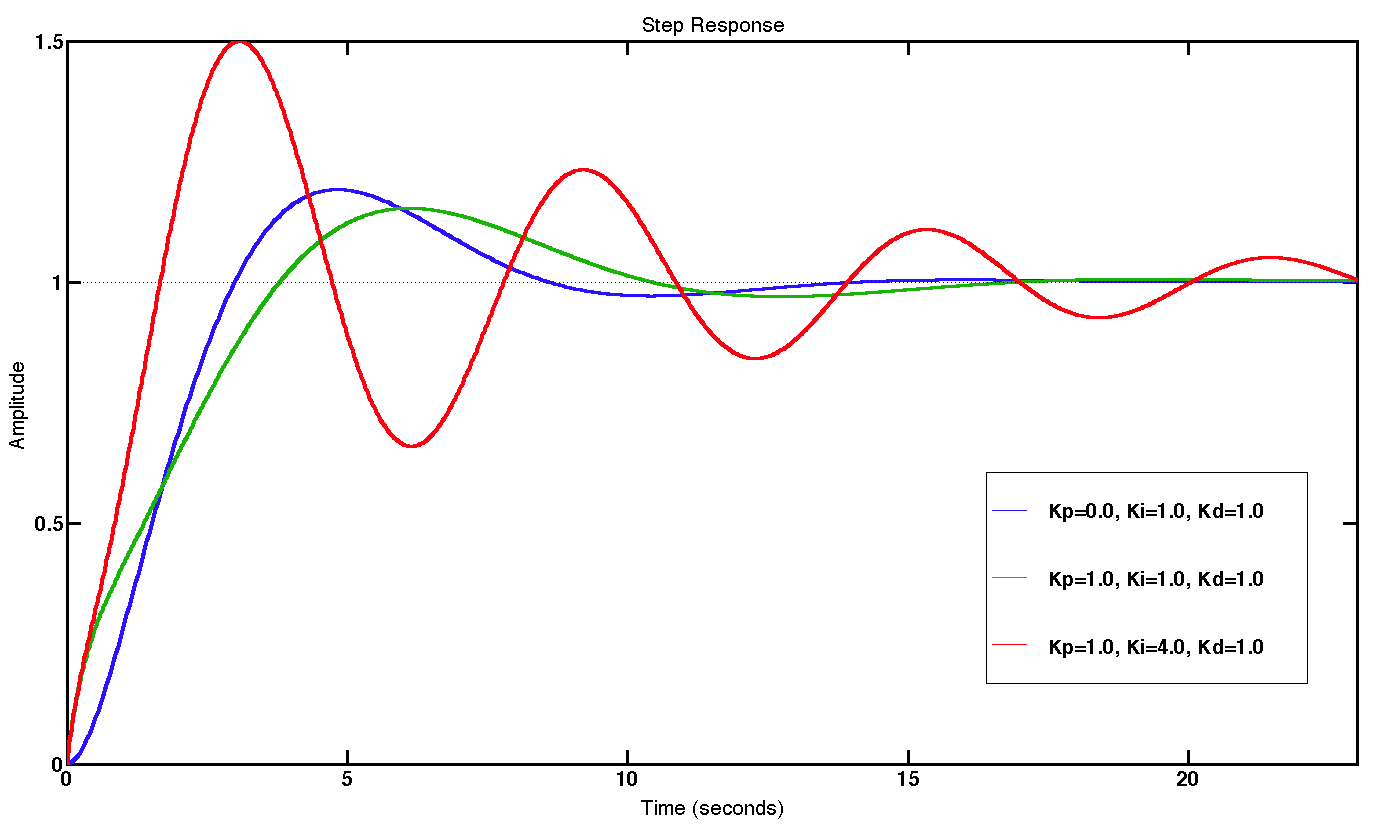
\includegraphics[width=\textwidth]{Figuras/pid_resposta}
\caption{Resposta do sistema em função dos parâmetros $K_p$, $K_i$ e $K_d$}
\label{fig:pid_respostal}
\end{figure}

O termo Integral atua na resposta de forma proporcional tanto ao valor do erro como ao tempo de duração deste erro, já que, como pode ser observado na equação \ref{eq:pid}, $\int^t_0{e\left(t\right)dt} $  é a área do gráfico do valor do erro em função do tempo. Os efeitos do termo $K_I$ no sistema são similares do $K_P$, também podendo levar a oscilações e instabilidades no sistema caso este seja muito alto. Como este termo responde ao erro acumulado, não existe o problema de baixa atuação quando $e(t)$ é pequeno e, portanto não leva a efeitos de erro residual no estado estacionário.

O termo derivativo responde em função da variação do erro $e(t)$ em função do tempo. Por isto, ele prevê a posição futura de $e(t)$ e com isto diminui o tempo que o sistema demora para chegar ao estado estacionário. Este termo deve ser empregado com cuidado pois em situações não ideais, as medidas das variáveis de interesse do sistema estejão sujeita a erros e flutuações como ruídos. Tais erros de medida podem gerar um grande valor da derivada de $e(t)$ e portanto gerar instabilidade no sistema. Por este motivo, sempre é ideal que os sensores possuam uma instrumentação eletrônica adequada, com filtros que evitem este problema.

\subsection{Automação}

Para que os conceitos de controle discutidos previamente possam funcionar em tempo real, as ações devem ser tomadas automaticamente pelo sistema. Portanto a automação é muito mais que uma forma de reduzir o número de trabalhadores braçais. 
Segundo \citet{process-monitoring-online}, os objetivos particulares da indústria de alimentos para a utilização de automação são: 

\begin{itemize}
  \item Qualidade e Confiabilidade.
  \item Segurança Alimentar.
  \item Flexibilidade e Manutenção.
  \item Implementação. 
  \item Aquisição de dados.
\end{itemize}

A qualidade, a confiabilidade e a segurança alimentar já foram discutidas nos benefícios do controle de processo. A flexibilidade e a manutenção são facilitados pela automação, pois numa planta de produção de alimentos, muitos produtos dividem os mesmos equipamentos, portanto a vantagem está em alterar facilmente o sistema para a produção de vários produtos. 

A aquisição de dados ajuda a melhorar o sistema, observando as respostas dos atuadores em várias circunstâncias e verificando os pontos que podem ser aprimorados. O monitoramento dos dados pode servir também como uma forma de alerta para evitar problemas na produção.


\section{Modelagem Matemática e Simulação na Indústria de Alimentos}\label{diffinitas}

A modelagem matemática é a descrição de um sistema real através de equações matemáticas, de forma que, através destas equações possam ser entendidos os efeitos de diferentes componentes do sistema bem como prever o comportamento deste diante de diferentes cenários. A modelagem matemática é a base das ciências naturais, das ciências sociais e da engenharia, já que podem ser testadas, validadas ou refutadas, passando pelo crivo do método científico. Do ponto de vista da Engenharia, o objetivo é analisar e otimizar sistemas, sendo que a descrição matemática do mesmo possibilita que testes sejam feitos através de simulações, economizando tempo e dinheiro. 

Na indústria de alimentos, os principais sistemas específicos a serem modelados são os relacionados a segurança alimentar, como crescimento bacteriano \citep{bacteriano}, os processos de contaminação \citep{contaminacao} e o processo de aquecimento/cozimento de alimentos, já que estes representam um alto gasto energético \citep{modelling-heat-bread} e pequenas alterações no perfil de temperatura do alimento podem  significar grandes mudanças sensoriais e perda do produto \citep{computer-aid}. 

Como o perfil de temperatura é extremamente importante para a qualidade do produto final, muitos estudos foram realizados com o intuito de modelar o processo de aquecimento em fornos. \citet{bread-baking} estudaram o processo interno de assamento levando em consideração o transporte de calor e de massa que ocorrem no interior do forno e dentro do alimento. O aquecimento do forno também foi estudado por \citet{modelling-heat-bread}, que estudaram os processos de transferência de calor e massa que ocorrem dentro de um forno linear tipo esteira com áreas de aquecimento inferior e superior e zonas de exaustão de ar. Tal tipo de forno é o mais comum na produção de pães e biscoitos e por este motivo este tipo de estudo ajudou a projetar fornos mais eficientes e que garantam o perfil de temperatura de forma mais adequada. Ainda em fornos tipo esteira, \citet{numerical-gas-flow} estudaram a velocidade do gás e o processo de convecção e \citet{cfd-modeling} realizaram simulações de dinâmica de fluido para resolver as equações do processo térmico dentro do forno.

\subsection{Transferência de Calor}

O processo de transferência de calor pode ser modelado aplicando um dos princípios mais básicos da Física, a conservação da Energia (E). O problema geral consiste em resolver a equação advinda da conservação de Energia para encontrar a temperatura em todos os pontos do sistema em função do tempo, ou seja, encontrar $T(x,y,z,t)$. Utilizando o princípio da conservação de Energia à um elemento infinitesimal de área podemos encontrar tal relação. Desta forma, podemos escrever a equação \ref{eq:energia}:

\begin{equation}\label{eq:energia}
E_{adicionada} = E_{entra} - E_{sai} + E_{'gerada'}
\end{equation}

Onde a Taxa de acúmulo de Energia é a derivada parcial da Energia em relação ao tempo e pode ser relacionada a temperatura através do Calor Específico pela equação \ref{eq:taxa-acumulo}.

\begin{equation}\label{eq:taxa-acumulo}
\frac{\partial U}{\partial x} \cdot m = \rho \cdot c_{p} \cdot \frac{\partial T}{\partial t}
\end{equation}

Onde $U$ é a energia interna por unidade de massa, $m$ é a massa, $\rho$ a densidade e $c_p$ é o calor específico à pressão constante.

A quantidade de Energia que entra menos a que sai em um elemento infinitesimal, em coordenadas cartesianas pode ser escrita utilizando a expansão em Série de Taylor (equação \ref{eq:taxa-entra-sai}), utilizando apenas o termo de primeira ordem.

\begin{equation}\label{eq:taxa-entra-sai}
E_{adicionada} = - ( \frac{\partial q_x}{\partial x} \cdot dx + \frac{\partial q_y}{\partial y} \cdot dy + \frac{\partial q_z}{\partial z} \cdot dz )
\end{equation}

Levando em consideração que o calor $q_x = -k \cdot (dy \cdot dz) \cdot \frac{\partial T}{\partial x}$, e que $q_y$ e $q_z$ tem o mesmo formato, podemos substituir na equação \ref{eq:energia} e então temos a equação \ref{eq:diferenca-final}.

\begin{equation}\label{eq:diferenca-final}
E_{entra} - E_{sai} = \frac{\partial}{\partial x} \cdot (k \cdot \frac{\partial T}{\partial x}) + \frac{\partial}{\partial y} \cdot (k \cdot \frac{\partial T}{\partial y}) + \frac{\partial}{\partial z} \cdot (k \cdot \frac{\partial T}{\partial z})
\end{equation}

Por último, temos o termo de “geração” de energia (equação \ref{eq:gerada}), que pode ser decorrente de reações químicas, sendo positivo para exotérmicas e negativo para endotérmicas ou também energia eletromagnética absorvida, como por exemplo micro-ondas. 

\begin{equation}\label{eq:gerada}
E_{gerada} = \dot{q}
\end{equation}

Com isto, temos a equação geral da transferência de calor, que em coordenadas cartesianas é dada pela equação \ref{eq:geral}.

\begin{equation}\label{eq:geral}
\rho \cdot c_{p} \cdot \frac{\partial T}{\partial t} = \frac{\partial}{\partial x} \cdot (k \cdot \frac{\partial T}{\partial x}) + \frac{\partial}{\partial y} \cdot (k \cdot \frac{\partial T}{\partial y}) + \frac{\partial}{\partial z} \cdot (k \cdot \frac{\partial T}{\partial z}) +  \dot{q}
\end{equation}

Para se encontrar $T(x,y,z,t)$ deve-se resolver a equação \ref{eq:geral}, aplicadas as condições conhecidas do problema em questão, que são chamadas condições de contorno. Porém, como a equação \ref{eq:geral} é uma EDP (Equação Diferencial Parcial), na maioria dos casos reais ela não pode ser resolvida analiticamente e por isto algum tipo de aproximação deve ser feita. 

Uma forma de se revolver este tipo de problema é nos casos em que alguma simetria, geométrica ou de condições de contorno, possibilitem algum tipo de solução analítica. Outra maneira de contornar o problema da resolução da EDP é desconsiderar termos menos significativos, que podem muitas vezes facilitar muito a solução da equação. Um exemplo clássico é a solução da equação de calor no estado estacionário, onde é considerado que  variação do perfil de temperatura em função do tempo é desprezível e portanto a solução que se quer encontrar, $T(x,y,z,t)$, passa a não ser mais função de t e então temos $T(x,y,z)$. Com isto, a equação \ref{eq:geral} é drasticamente simplificada já que $\frac{\partial T}{\partial t} = 0$ e então temos a equação \ref{eq:simplificada}.

\begin{equation}\label{eq:simplificada}
 k \cdot (\frac{\partial^2}{\partial x^2} + \frac{\partial^2}{\partial y^2} +  \frac{\partial^2}{\partial z^2}) T + \dot{q} = 0 
\end{equation}

Mesmo com a  equação \ref{eq:simplificada}, dependendo de quem for $\dot{q}$ e também da geometria, pode não ser possível resolver o problema analiticamente. Nestes casos, existem vários métodos computacionais que podem ser utilizados.

\subsection{Simulação de Processos Térmicos}

Como na maioria dos casos reais não existe uma solução analítica para a equação da transferência de calor, os métodos numéricos são comumente utilizados para se obter uma aproximação satisfatória das equações. Existem vários métodos computacionais que podem ser utilizados, como por exemplo o método dos elementos finitos, das diferenças finitas e Lattice Boltzman. Além destes métodos numéricos, outra forma de encontrar a solução da equação da transferência de calor é utilizando Eurística, baseando-se em conhecimento experimental prévio do sistema ou em princípios de Mínima Ação. Neste tipo de método podemos destacar  as Redes Neurais e o Algoritmo Genético, respectivamente.

\subsubsection{Diferenças Finitas}

O método das diferenças finitas é uma técnica utilizada para encontrar soluções aproximadas de uma ou de um conjunto de equações diferenciais. Basicamente, o método consiste em substituir a derivada de uma função pela equação \ref{eq:derivada}, utilizando o teorema fundamental do cálculo, com um valor pequeno de $\Delta x$. Desta forma, quanto menor for o valor de $\Delta x$, maior será a precisão do cálculo uma vez que o limite de $\Delta x$ tendendo a zero resulta no valor exato da derivada. 

\begin{equation}\label{eq:derivada}
\frac{\mathrm{d} }{\mathrm{d} x}y(x) = \frac{y(x + \Delta x) - y(x)}{\Delta x}
\end{equation}

Além disso, o método também discretiza o espaço, em uma série de pontos separados por uma distância $\Delta x$. Desta forma, o resultado é um conjunto de equações não diferenciais que podem ser resolvidas para encontrar a solução discretizada da equação.

Quanto menor for $\Delta x$, maior será a precisão do método, no entanto maior será a quantidade de equações e mais demorado será para encontrar a solução.

Depois que $y(x)$ foi discretizado em $k$ valores ($y_1$, $y_2$, ..., $y_k$), o conjunto de equações gerado pelo método tem o formato da equação \ref{eq:dif-discreta} no caso unidimensional e o conceito é similar para duas ou três dimensões. O conjunto de equações acopladas deverá ser resolvido para se encontrar a temperatura em todos os pontos num instante t. 

\begin{equation}\label{eq:dif-discreta}
y_k = \frac{y_{k+1} + y_{k-1} + \dot{q_k} \cdot (\Delta x)^2}{2}
\end{equation}

Como geralmente existe uma grande quantidade de equações, vários métodos de resolução podem ser aplicados, com vantagens e desvantagens que dependem da geometria, quantidade de dimensões e tipo de condições de contorno presentes no problema. As principais a serem destacadas são o método de Jacobi, Gauss-Seidel, Sucessive Over-Relaxacion (SOR) e o método direto. 

No método direto, é montada uma equação matricial no formato $ \mathbf{A} \cdot \mathbf{x} = \mathbf{B}$, onde $\mathbf{A}$ é a matriz dos coeficientes das equações acopladas, $\mathbf{x}$ é a matriz das incógnitas (temperatura) e $\mathbf{B}$ é uma matriz conhecida de valores dada pelas condições de contorno do problema e para o caso unidimensional, o formato da equação matricial é dado pela equação \ref{eq:matricial}, onde foi escolhido k=5 para exemplificar o problema. 

\begin{equation}\label{eq:matricial}
 \begin{bmatrix}
    -2 & 1 & 0 & 0 & 0  
\\  1 & -2 & 1 & 0 & 0
\\  0 & 1 & -2 & 1 & 0
\\  0 & 0 & 1 & -2 & 1
\\  0 & 0 & 0 & 1 & -2
\end{bmatrix}  \cdot \begin{bmatrix}
    T_1 
\\  T_2
\\  T_3
\\  T_4
\\  T_5
\end{bmatrix} = -(\Delta x)^2  \begin{bmatrix}
    \dot{q}_1 
\\  \dot{q}_2
\\  \dot{q}_3
\\  \dot{q}_4
\\  \dot{q}_5
\end{bmatrix} - \begin{bmatrix}
    T_{esquerda}
\\  0
\\  0
\\  0
\\  T_{direita}
\end{bmatrix}
\end{equation}
Onde A e B representam as temperaturas conhecidas nas laterais esquerda e direita de $T_1$ e $T_5$ respectivamente e $\dot{q_1}$, ..., $\dot{q_5}$ representam o calor sendo adicionado ou removido no instante t nos pontos discretizados do eixo x.

O conhecimento da temperatura nas laterais, que é uma codição de contorno chamada condição de Dirichlet, e o conhecimento do calor adicionado no sistema, que é uma condição de contorno de Neumann, precisam ser conhecidas para se encontrar a solução particular do sistema.

Para encontrar a matriz das incógnitas, é preciso simplesmente encontrar a inversa de $\mathbf{A}$. Este processo pode ser computacionalmente custoso para matrizes muito grandes porém como a matriz $\mathbf{A}$ sempre é uma matriz esparsa, este problema pode ser contornado. No caso unidimensional, já que segundo a equação \ref{eq:dif-discreta}, os elementos desconhecidos $T_a$ estão relacionados apenas com os seus vizinhos $T_{k+1}$ e $T_{k-1}$,  a matriz $\mathbf{A}$ é sempre tridiagonal, o que facilita muito a resolução do problema \citep{tridiagonal}, já que reduz o número de iterações da ordem de $n^3$ para $n$, se considerarmos uma matriz $n \times n$. Para o caso 2D e 3D, teremos matrizes com blocos tridiagonais, simetria que também ajuda na inversão da matriz.

Além do método de resolução direta, existem formas iterativas de se resolver o conjunto de equações acopladas. Tanto o método de Jacobi, Gauss-Seidel e SOR consistem em resolver ponto a ponto as equações, partindo de um "chute inicial" para a temperatura. Este cálculo é reiterado até que os valores da temperatura atinjam uma estabilidade e não se alterem mais. 

Os três métodos citados acima variam na forma com que é feita a resolução das equações. No método de Jacobi (equação \ref{eq:jacobi}), o calculo de $T_k^i$ é dado em função de  $T_{k+1}^{i-1}$ e $T_{k-1}^{i-1}$, ou seja, em função da iteração passada. 

\begin{equation}\label{eq:jacobi}
T_k^i = \frac{T_{k+1}^{i-1} + T_{k-1}^{i-1} + \dot{q_k} \cdot (\Delta x)^2}{2}
\end{equation}
Onde $i$ representa a iteração e $T_k^1$, é um "chute" inicial da temperatura para todo $k$. A equação \ref{eq:jacobi} é resolvida para todos os valores de $k$, repetidamente para $i=2$, $i=3$, e assim por diante até que não haja mais alterações significativas nos valores de $T_k$ em relação a iteração anterior, indicando que o algoritmo convergiu e foi encontrada a solução de $T_k$ para todo $k$.

O método de Gauss-Seidel (equação \ref{eq:gauss-seidel}), é um aprimoramento do anterior, e o cálculo de $T_{k}^i$ é feito em função de $T_{k+1}^i$ e $T_{k-1}^i$, e não da iteração anterior ($i-1$), o que acelera o processo de convergência. 

\begin{equation}\label{eq:gauss-seidel}
T_k^i = \frac{T_{k+1}^{i} + T_{k-1}^{i} + \dot{q_k} \cdot (\Delta x)^2}{2}
\end{equation}

No método SOR, a atualização do valor $T_k^i$ leva em conta também um parâmetro chamado parâmetro de relaxação que aumenta a velocidade de convergência. Primeiramente, é calculada a diferença entre $T_k^{i-1}$ e $T_k^i$ encontrado pelo método de Gauss-Seidel. Essa diferença é então amplificada pelo fator $w$, o parâmetro de relaxação, sendo que $ 1 < w < 2$. Finalmente o valor $T_k^i$ real é encontrado, como é mostrado na equação \ref{eq:sor}.

\begin{equation}\label{eq:sor}
T_k^i(sor) = T_k^{i-1} + w \cdot ( T_k^i(Gauss-Seidel) - T_k^{i-1} )
\end{equation}


\section{Sistemas Embarcados}\label{embarcados}

Sistemas embarcados são dispositivos eletrônicos com poder computacional que fazem parte de um sistema mecânico/eletrônico maior. Estes dispositivos interagem com outras partes do sistema realizando operações lógicas em tempo real, assim como um PC (computador pessoal), porém os periféricos de entrada e saída não são de propósito geral e cada sistema embarcado é feito para a sua função específica e, portanto geralmente possui menor custo, tamanho e gasto energético. Eles são encontrados em quase todos os dispositivos eletrônicos atuais, desde controles remotos de televisão, televisões, rádios, semáforos, radares, fornos de micro ondas e etc.

Dentro da indústria de alimentos, os sistemas embarcados mais importantes são os que controlam o processo de produção. Estes sistemas devem estar conectados aos sensores e a outros sistemas da indústria, processando os dados recebidos e tomando as decisões de controle que são enviadas aos atuadores. As alternativas de sistemas embarcados para este tipo de controle são os CLP’s (Controles Lógico Programáveis), microcontroladores, computadores e sistemas mistos com processamento distribuído. Segundo uma pesquisa de \citet{survey-automation}, 88 \% das indústrias de alimentos utilizam os CLP’s como principal forma de controle e em apenas 6 \% predominam sistemas distribuídos. Esta pesquisa também revelou que uma grande gama de marcas e sistemas comerciais são utilizados, inclusive dentro de uma mesma empresa, o que dificulta uma integração mais inteligente dentro do sistema.

Apesar do grande uso de CLP’s dentro das indústrias de alimentos,  estes dispositivos não tiveram a mesma evolução que os computadores portáteis e dispositivos móveis tiveram nos últimos 15 anos, com um grande aumento no processamento e redução no preço. Por este motivo o desenvolvimento de sistemas de controle baseados em microcontroladores tem crescido muito, com placas que podem realizar as mesmas operações com tamanho e custo reduzido \citep{clp-microcontrolador}. Para controles mais complexos, que exijam um maior processamento de dados, os sistemas de computação de baixo custo baseados em hardwares similares a tablets e celulares também é uma alternativa emergente. 

\subsection{Microcontroladores}

Microcontroladores são pequenas unidades de processamento que possuem todos os seus elementos de processamento e memória em um único chip e, portanto podem operar sem a necessidade de periféricos. Esta é a principal diferença entre um microcontrolador e um microprocessador, como os que são encontrados nos computadores. Por possuir todas as unidades em um único chip, seu processamento e memória são em geral muito inferiores a de um computador, porém as vantagens estão na quantidade de energia utilizada, tamanho e robustez. 

Os microcontroladores surgiram na década de 1970 e tiveram um enorme avanço até o momento. Atualmente, existem centenas de empresas que produzem microcontroladores e suas especificações variam de acordo com o objetivo do mesmo dentro do sistema, podendo ir de chips minúsculos e baratos com velocidade da ordem de kHz e apenas um pino digital de entrada e saída a microcontroladores ARM (Advanced RISC Machine – Máquina RISC Avançada), que possuem processamento e arquitetura superior aos microcontroladores RISC tradicionais, atingindo processamento da ordem de GHz. 

\subsubsection{Arduino}

Dentro deste conceito de hardware livre surge a plataforma Arduino (figura \ref{fig:arduino}). Esta plataforma foi concebida em 2005 por uma equipe sediada na Itália liderada pelo pesquisador Massimo Banzi, que queria ensinar eletrônica e programação de computadores a alunos de design, para que eles usassem em seus projetos de arte, interatividade e robótica \citep{arduino-araujo}. O intuito da equipe era desenvolver uma plataforma para introduzir os conceitos de eletrônica e programação para leigos de forma intuitiva, simplificada e de baixo custo \citep{arduino-barrett}.

\begin{figure}[H]
\centering
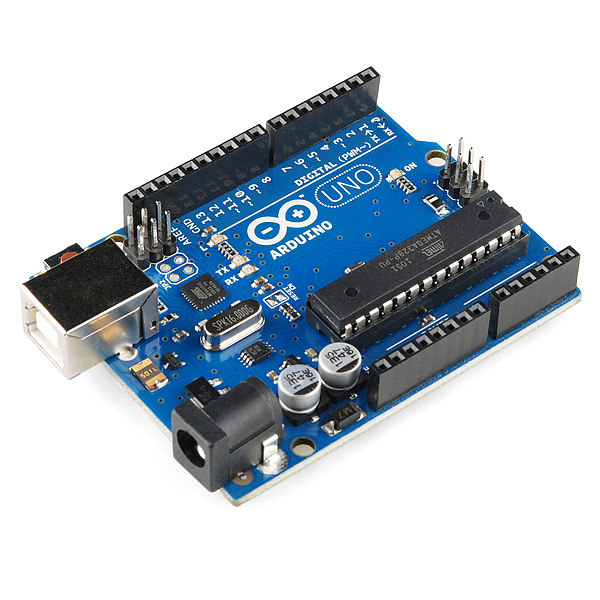
\includegraphics[width=\textwidth]{Figuras/arduino}
\caption{Arduino Uno R3 – Principal placa da plataforma Arduino, com Atmega328pu e Comunicação USB}
\label{fig:arduino}
\end{figure}

O Arduino é uma plataforma de placas microcontroladoras que permite entrada de dados de sensores e comunicação digital e saídas de dados e sinal elétrico que possibilita acionar motores, LEDs e outros dispositivos. A principal placa da linha Arduino, o Arduino Uno utiliza um microcontrolador \textregistered{Atmel} da linha Atmega com um oscilador de 16 MHz externo, um regulador de tensão de 5 V, botão de reset, plugue de alimentação, pinos conectores, e alguns LEDs para facilitar a verificação do funcionamento. A conectividade é feita diretamente por uma porta USB, tanto para gravar os programas quanto para comunicação serial. Além disso, a porta USB pode também fornecer a alimentação de 5 V para a placa.

A gravação dos programas na placa é controlada por um chip que faz a conversão USB para Serial, sendo nos primeiros modelos o CHIP FT232RL, que na terceira revisão do Arduino UNO foi substituído por um microcontrolador Atmega16U2, que tem o papel exclusivo de ser a interface entre a porta USB e o Arduino \citep{arduino-testes}. Este conceito é uma das chaves do sucesso da plataforma, já que a gravação dos programas pode ser feita diretamente na placa, não exigindo um gravador externo como a maioria dos microcontroladores do mercado. Isto viabilizou a utilização de microcontroladores por pessoas que não tem acesso a um laboratório de eletrônica.

A programação do microcontrolador utiliza uma interface integrada de desenvolvimento (IDE) baseada na IDE da linguagem Processing, que é uma versão simplificada (mas não menos poderosa) da linguagem C/C++ \citep{arduino-buechley}. Esta Linguagem foi desenvolvida em 2001 no laboratório de mídia do MIT (Massachusetts Institute of Technology), e esta licenciada sobre a licença GPL e LGPL (General Public License - Licença Pública Geral), sendo completamente open source e cross plataforma, podendo ser utilizado nos sistemas Windows, Linux e Mac OS. O \textit{Processing} foi desenvolvido inicialmente para facilitar o uso de programação por artistas e ensinar programação de forma simples e visual \citep{processing} e pela sua facilidade é utilizado atualmente por milhões de pessoas desde o ensino a prototipagem e produção de softwares.

Outra facilidade da plataforma Arduino é a padronização dos pinos de Entrada e Saída, possibilitando que uma série de circuitos de expansão, chamados de Shields, possam ser utilizados com as placas, dando funções extras ao microcontrolador, como comunicação Bluetooth, wi-fi, GSM, Relês entre outros. Estes Shields, assim como as próprias placas, podem ser produzidos por qualquer companhia já que o Arduino é um hardware livre. Com isto, com a popularização das placas, mais sensores, Shields e periféricos são produzidos para abastecer o ecossistema, o que torna o Arduino ainda mais popular, fazendo disto um ciclo positivo \citep{arduino-livro}. O mesmo ciclo ocorre com a disponibilização de projetos com código aberto e dessa forma, quanto maior for o número de usuários da plataforma, maior será a quantidade de projetos livres e suporte disponíveis para o ecossistema.

\subsection{Computação de Baixo Custo}

Com o avanço e desenvolvimento de novos hardwares com mais memória e processamento e, principalmente devido à corrida tecnológica dos dispositivos móveis, surgiu nos últimos anos a computação de ultra baixo custo (Ultra Low Cost Computing – ULCC), que basicamente utiliza o hardware de smartphones e periféricos de entrada e saída em uma única placa \citep{low-cost-computing}. Vários projetos tem se desenvolvido neste sentido, entre eles podemos citar o Beaglebone, Galileu Board, Raspberry Pi, Arduino Yun e PcDuino. Tais projetos entregam placas de baixo custo (de 20 a 70 dólares) que possibilitam aplicações em várias áreas como automação, robótica, equipamentos médicos \citep{raspberry-pesquisa}, ensino de computação e programação, aquisição dinâmica de dados, servidores web, monitoramento remoto e até controle de satélites \citep{raspberry-embedded}, entre outras aplicações. 

Existem vários modelos de computadores em uma única placa, que diferem nas suas especificações de preço, processamento, sistema operacional e tipo de licença. Levando em conta o preço, licença e a quantidade de usuários, o Raspberry pi é a placa que mais se destaca no mercado atualmente.

\subsubsection{Raspberry Pi}

O Raspberry pi é um computador em uma única placa do tamanho de um cartão de crédito (figura \ref{fig:raspberry}), desenvolvido pela Raspberry Pi Foundation, que se iniciou com o intuito de promover o ensino básico de computação em escolas com baixo custo. O Raspberry Pi, modelo B é produzido em um único chip broadcom BCM2835, com um processador ARM de 700 MHz e 512 Mb de memória RAM. A memória física fica em um cartão SD de até 32 Gb e suporta uma série de sistemas operacionais baseados em Linux e a distribuição oficial da Raspberry Pi Foundation é um Linux Debian chamado wheezy. Este modelo possui duas entradas USB, uma porta Ethernet, uma saida HDMI, uma saída RCA, uma saída de vídeo e oito pinos GPIO (General Purpose Input/Output - Pinos de entrada/saída de propósito geral).

\begin{figure}[H]
\centering
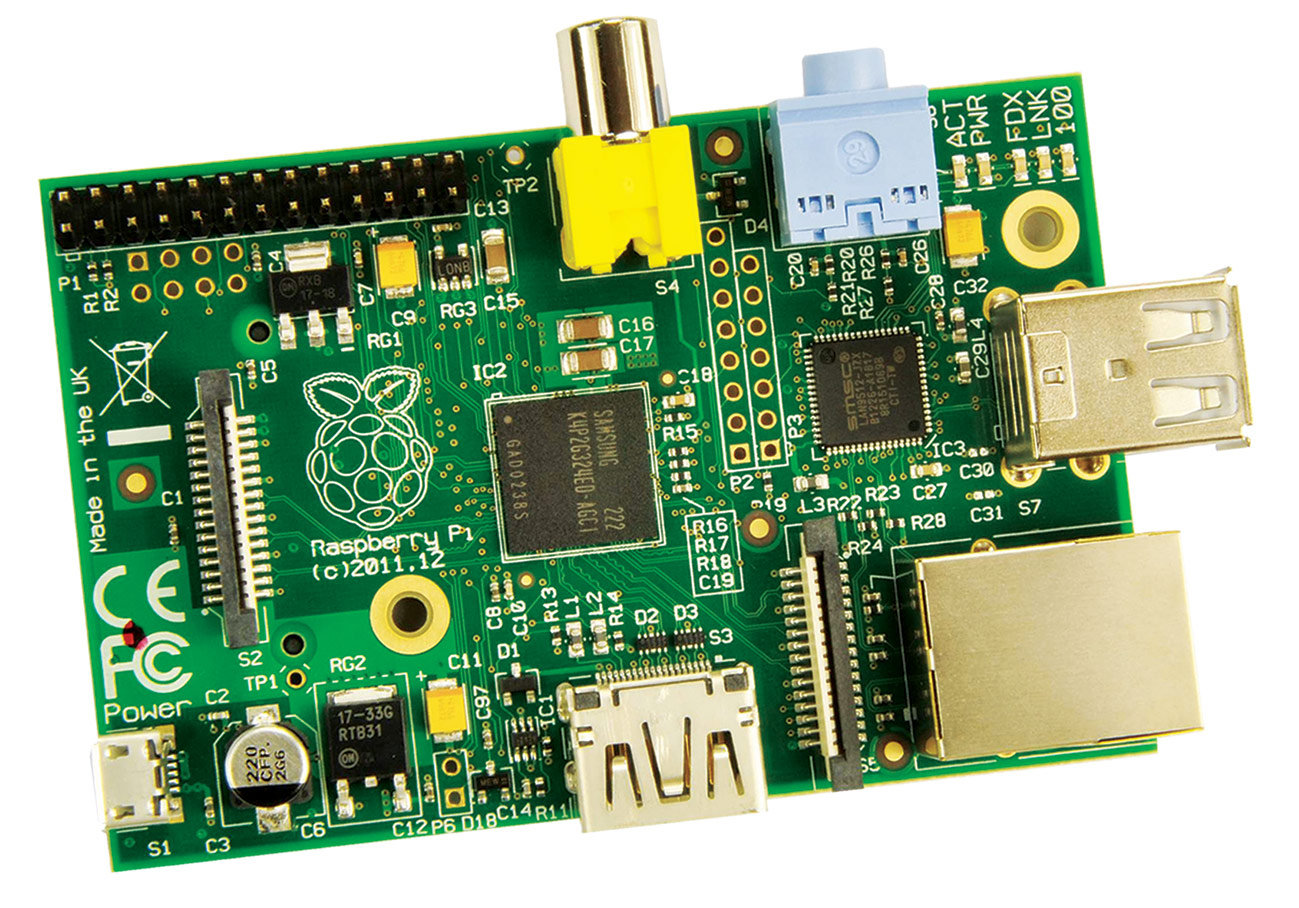
\includegraphics[width=\textwidth]{Figuras/raspberry}
\caption{Raspberry pi – Modelo B}
\label{fig:raspberry}
\end{figure}

O projeto foi concebido em 2006 como uma forma barata e simples de ensinar computação, programação e eletrônica às crianças. Em 2008 o projeto saiu do papel com o modelo A, que possuía 256 Mb de memória RAM (Random Access Memory) e uma entrada USB. Este modelo recebeu um upgrade em 2011, contando agora com uma memória de 512 Mb e duas entradas USB. Por ser um projeto totalmente open-source ele usa uma distribuição Unix com licença GNU além de um hardware aberto. Com isto, o Raspberry Pi ganhou muitos adeptos rapidamente, sendo utilizado atualmente em várias áreas como ensino, processamento e clusters, webservers e uma série de projetos embarcados.

Na área da educação, a placa tem sido utilizada devido ao seu baixo custo (aproximadamente 35 dólares) e também por ser uma maneira mais acessível do usuário entender e manipular o hardware. Nesta ultima década, dispositivos computacionais tem se tornado equipamentos fechados em que o usuário o encara como unidades lacradas de alumínio ou plástico, sem ideia do que esta dentro. Neste sentido, o Raspberry Pi possibilita ao usuário o entendimento a alterações no hardware assim como do software, já que utiliza um Linux que possui várias vantagens didáticas. Baseado nestas ideias, alguns projetos para ensino de computação em comunidades carentes utilizam esta plataforma como uma alternativa barata e poderosa, como por exemplo, o projeto de \citet{raspberry-data}.

Além de projetos educacionais, o Raspberry Pi é utilizado também em projetos de pesquisa de ponta, como por exemplo o satélite CCRMA \citep{raspberry-embedded} que envia placas para controlar pesquisas científicas em satélites. Na área da medicina, existem vários projetos de controle e desenvolvimento de equipamentos baratos \citet{raspberry-pesquisa}.

No novo conceito de IoT (Internet of Things - Internet das Coisas), desenvolvido por Kevin Ashton em 2009, num mundo onde objetos físicos estão integrados a uma rede de informações, os objetos se tornam “inteligentes” e podem interagir com o resto da rede. Neste cenário, computadores pequenos e de baixo custo como o Raspberry Pi são extremamente importantes já que podem servir como unidades móveis de processamento de dados \citep{raspberry-pesquisa} bem como receber e processar dados de sensores numa rede multi-agente \citep{raspberry-data}.










































    \chapter{Objetivo}\label{objetivo}

Este trabalho tem como objetivo testar a seguinte hipótese:

\textit{"É possível o controle e automação de um forno experimental tipo túnel com informações de sensores e simulação computacional em tempo real utilizando computação embarcada de baixo custo"}

Para testar esta hipótese os seguintes objetivos específicos foram \textcolor{blue}{(azul)} ou serão \textcolor{red}{(vermelho)} desenvolvidos:

\begin{itemize}

    \item \textcolor{blue}{Modelagem matemática do comportamento térmico do forno.}
  
    \item \textcolor{blue}{Simulação do comportamento térmico utilizando diferenças finitas.}
  
    \begin{itemize}
    
        \item \textcolor{blue}{Teste da velocidade de convergência da simulação em função de várias técnicas de diferenças finitas.}
    
        \item \textcolor{blue}{Teste de tempo de execução em função da linguagem em que o algoritmo foi implementado.}
    
        \item \textcolor{red}{Levantar o perfil térmico do forno com sensores embarcados e comparar com o perfil simulado para validação.}
    
    \end{itemize}

    \item \textcolor{blue}{Implementação de um controle PID baseado na resposta da simulação e do conhecimento do perfil de temperatura desejado para o biscoito.}   
   
    \begin{itemize}
    
        \item \textcolor{blue}{Desenvolvimento de um algoritmo de controle PID em função de Kp, Ki e Kd.} 
    
        \item \textcolor{red}{Obter a resposta impulsiva da temperatura no forno e 	calcular a função de transferência (Temperatura em função da 	potência).}

        \item \textcolor{red}{Encontrar o Kp, Ki e Kd ótimos para o controle do forno.}
        
        \item \textcolor{red}{Comparar a função de transferência obtida com o perfil térmico em várias situações de operação do forno.}
    
    \end{itemize}

    \item \textcolor{blue}{Desenvolvimento de um software com interface gráfica amigável para controle do forno.}
    
    \item \textcolor{red}{Teste do sistema em vários dispositivos embarcados.}
 
\end{itemize}




    \chapter{Materiais}\label{materiais}

\section{Forno de esteira em escala}\label{modelo-do-forno}

Todo o sistema de controle, as modelagens matemáticas e  as simulações foram desenvolvidas baseadas no forno de esteira em escala reduzida localizado no LAFAC (Laboratório de Física Aplicada e Computacional), situado em Pirassununga, na Faculdade de Zootecnia e Engenharia de Alimentos da USP (figura \ref{fig:forno_real}). Este forno foi desenvolvido por \citet{arthur} e pelos pesquisadores do LAFAC como parte de um projeto de automação de uma linha de produção industrial (FAPESP 2009/07593-1).

\begin{figure}[H]
\centering
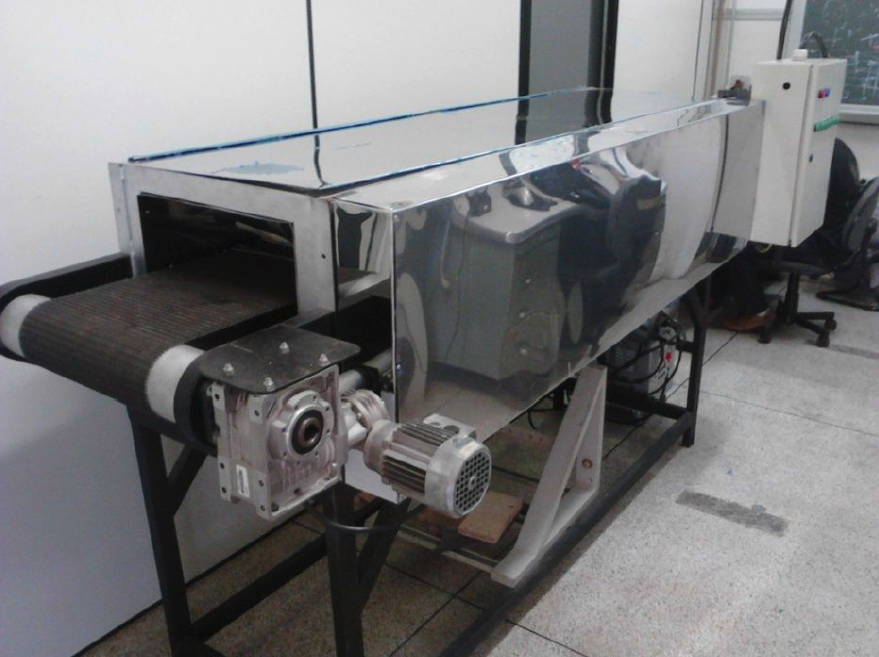
\includegraphics[width=\textwidth]{Figuras/forno_real}
\caption{Forno de esteira em escala - LAFAC}
\label{fig:forno_real}
\end{figure}

O forno possui 2,0 metros de comprimento por 0,5 metros de altura e largura, sendo revestido externamente por aço inox e placas de cerâmica refratária, como pode ser visto na figura \ref{fig:forno_frontal}. O espaço interno do forno possui  2,0 metros de comprimento por 0,4 metros de altura e largura, espaço este que possui duas áreas principais, o topo e o lastro, que estão separados pelas esteira de transporte. A esteira é circular e tanto a entrada, como a saída do forno são abertas.

\begin{figure}[H]
\centering
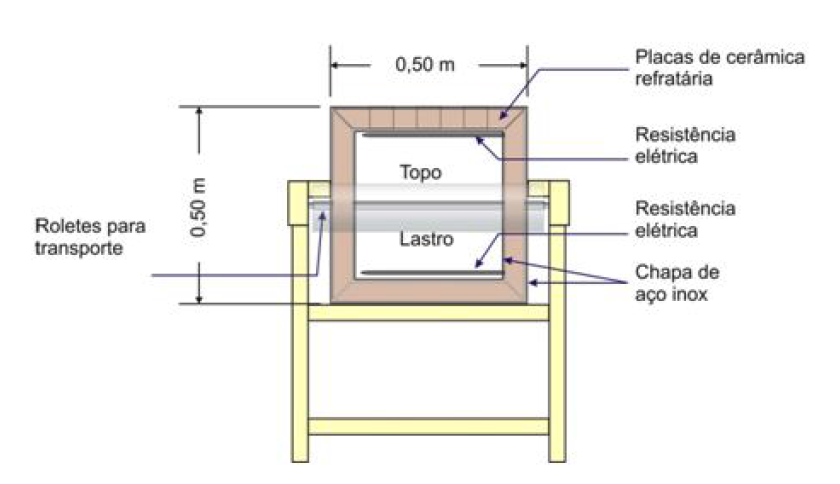
\includegraphics[width=\textwidth]{Figuras/forno_frontal}
\caption{Vista frontal forno. Adaptado de \citet{arthur}}
\label{fig:forno_frontal}
\end{figure}

O aquecimento do forno é feito por resistências que estão posicionadas ao longo da parte superior e inferior do forno de forma contínua. As ligações das resistências são separadas de forma a se controlar individualmente cada um dos 6 setores ilustrados pela figura \ref{fig:forno_esquema_lateral}, com os setores de 1 à 3 na parte superior e de 4 a 6 na parte inferior. 

\begin{figure}[H]
\centering
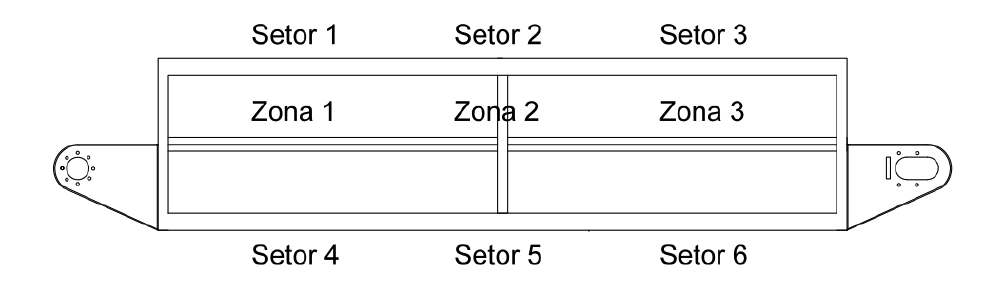
\includegraphics[width=\textwidth]{Figuras/forno_esquema_lateral}
\caption{Vista lateral do forno. Adaptado de \citet{arthur}}
\label{fig:forno_esquema_lateral}
\end{figure}

Seis sensores de temperatura termopar tipo K estão posicionados nos setores de 1 à 3 em ambos os lados do forno estão acoplados a amplificadores com compensação de junção fria AD595. Uma unidade controladora recebe os dados dos sensores por um barramento $I^2C$ e envia por radiofrequência as informações para uma estação de controle. As informações a respeito da velocidade da esteira e potência em cada uma das zonas de aquecimento também são recebidas por radiofrequência pela estação controladora.

 \section{Perfil de Temperatura no forno}
 
A unidade controladora recebe continuamente os dados da temperatura dos seis sensores localizados nas zonas 1, 2 e 3. Estes dados de temperatura, juntamente com a potência em cada uma das resistências formam as condições de contorno da simulação numérica, que calculará a temperatura em outros locais do forno. 

Para se comparar os valores calculados com a temperatura real em função da posição, um sensor termopar se deve mover dentro do forno. Como a temperatura do forno é muito acima da suportada pelos componentes eletrônicos em geral, um invólucro de cimento refratário foi utilizado para proteger o sensor e o circuito eletrônico adjacente (figura \ref{fig:envoltorio_sensor}).

\begin{figure}[H]
\centering
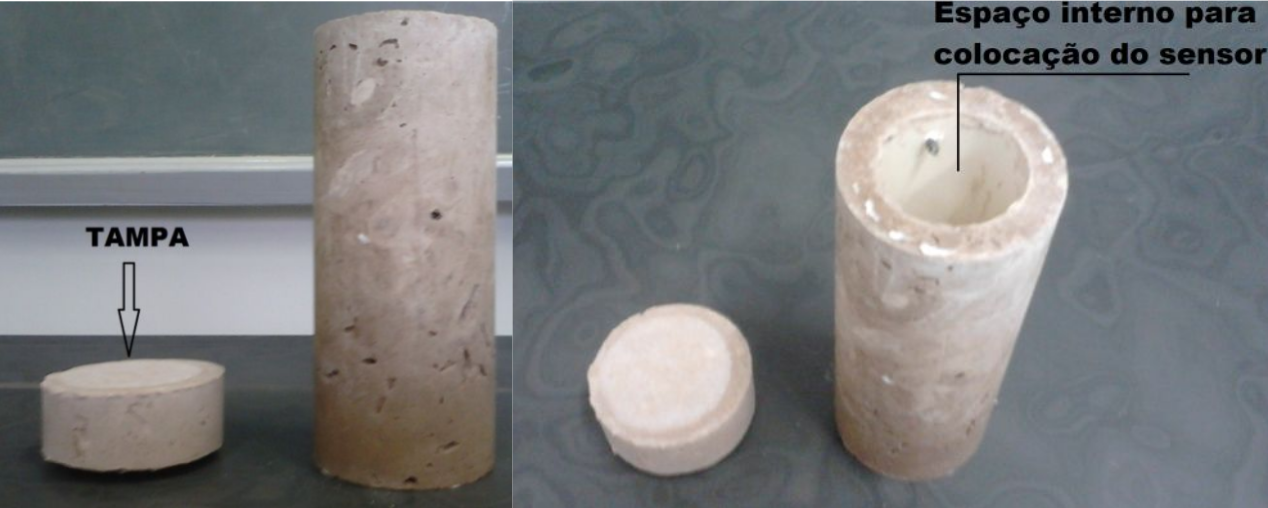
\includegraphics[width=\textwidth]{Figuras/envoltorio_sensor}
\caption{Envoltório refratário para sensor de temperatura embarcado (Figura \ref{fig:sensor_termeratura}). Adaptado de \citet{arthur}}
\label{fig:envoltorio_sensor}
\end{figure}

O circuito consiste em um termopar tipo K com um amplificador com compensação de junção fria AD595, cujos dados são recebidos por um microcontrolador PIC12F675 e enviados por um módulo transceptor de radiofrequência (figura \ref{fig:sensor_termeratura}), para que a informação possa ser coletada por um computador nas proximidades do forno.
 
\begin{figure}[H]
\centering
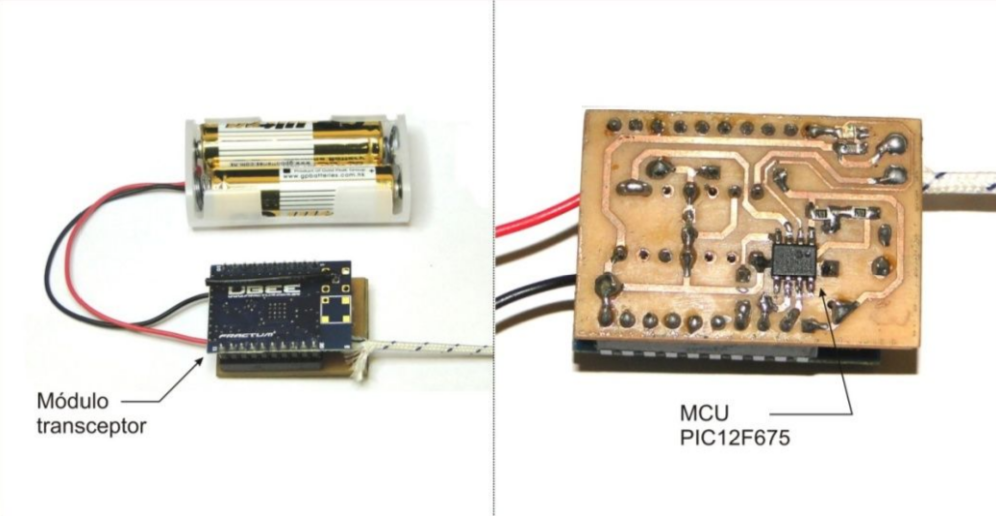
\includegraphics[width=\textwidth]{Figuras/sensor_termeratura}
\caption{Módulo transmissor com Sensor de temperatura microcontrolado. Adaptado de \citet{arthur}}
\label{fig:sensor_termeratura}
\end{figure}

O equipamento com o sensor, microcontrolador e transmissor de radio frequência mostrados pela figura \ref{fig:sensor_termeratura} foram encapsulados no envoltório de cerâmica da figura \ref{fig:envoltorio_sensor}, ficando apenas a junção do termopar no lado externo, como ilustra a figura \ref{fig:sensor_movel}.

\begin{figure}[H]
\centering
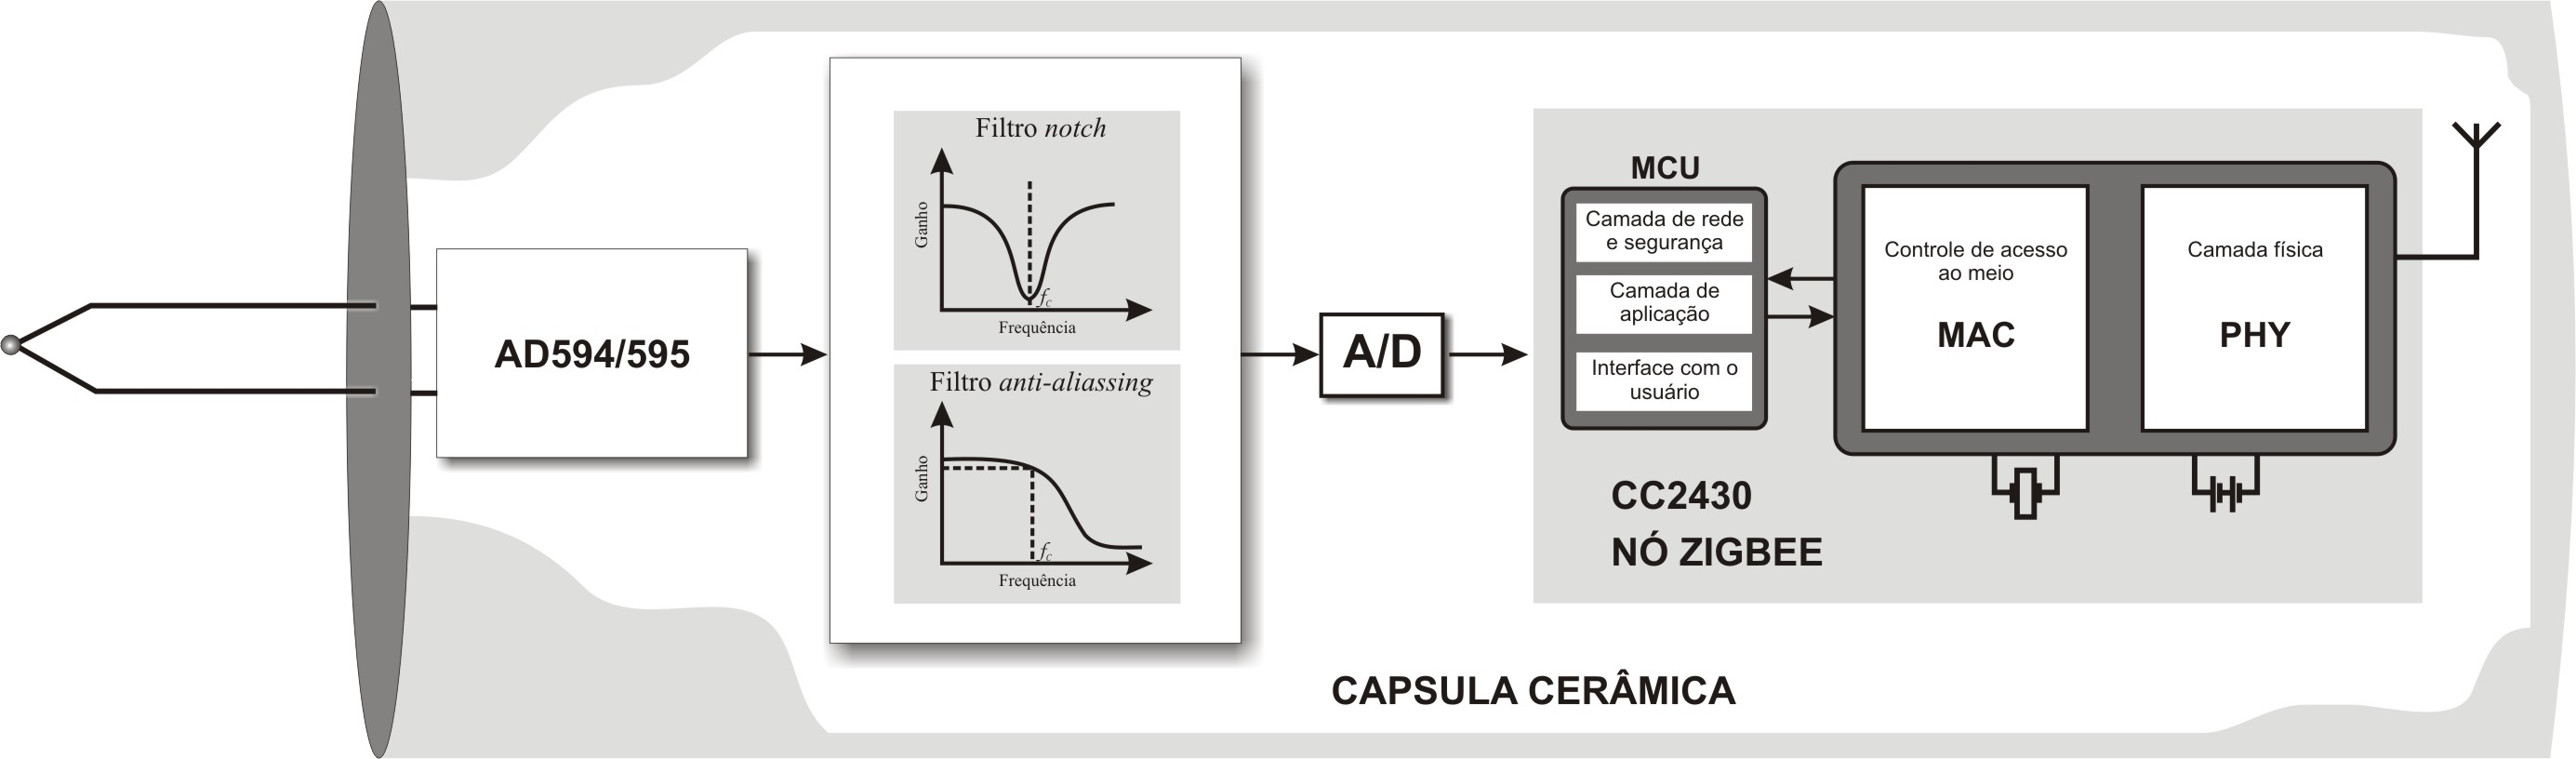
\includegraphics[width=\textwidth]{Figuras/sensor_movel}
\caption{Esquemático do sensor móvel embarcado no envoltório de cerâmica, com as funcionalidades do sensor: Amplificador e filtro, conversão analógico/digital e envio de dados por radiofrequencia}
\label{fig:sensor_movel}
\end{figure}

Alguns testes foram feitos com o sensor e o envoltório, mostrando que o processo desta metodologia, desenvolvida por \citet{arthur} funciona, dando uma noção qualitativa do comportamento da temperatura no forno em função da potencia nas zonas de aquecimento, porém mais experimentos devem ser feitos de forma sistemática para que os dados possam ser utilizados e comparados com os obtidos pela simulação. 
 
\section{Simulação da Temperatura}\label{simulação-temperatura}
 
As simulações numéricas foram feitas assumindo que a temperatura no interior do forno é dado pela equação \ref{eq:geral}, assumindo as simplificações de que não há deslocamento de ar significativo em um padrão diferente da difusão e que o estado estacionário é atingido rapidamente em comparação com as grandezas de tempo envolvidas nos processos de assamento. 

Assumindo o estado estacionário, em que $\frac{\partial T}{\partial t} = 0$, a equação a ser resolvida passa a ser a \ref{eq:simplificada} , que pode ser resolvida por diferenças finitas. Caso os resultados não sejam coerentes com os dados experimentais de temperatura dentro do forno, um novo modelo de simulação, envolvendo a circulação de ar e os efeitos da esteira será desenvolvido e testado.

\subsection{Diferenças finitas em uma Dimensão}

Para as simulações por diferenças finitas em uma dimensão, foram desconsideradas a altura e a largura do forno e levada em conta apenas a profundidade do mesmo. As equações de diferenças finitas foram resolvidas tomando como conhecida a temperatura nos três pontos dos sensores embutidos no forno e a potência irradiada pelas resistências.

O problema foi separado em duas partes, entre o sensor 1 e 2 e entre o sensor 2 e 3, de modo a utilizar como contorno externo a temperatura conhecida. As condições de contorno são portanto, de Dirichlet para a temperatura e de Neumann para o calor fornecido pelas resistências.


\subsubsection{Teste dos Algoritmos}\label{teste_alg}

Baseado nas condições de contorno descritas acima, foram desenvolvidos vários algoritmos para a resolução das equações de diferenças finitas em uma dimensão. Os algoritmos desenvolvidos estão apresentados no anexo \ref{alg:dif1d} e são baseados nos métodos de Jacobi, Gauss-Seidel, SOR e no método Direto. 

Com o intuito de se testar os algoritmos e verificar a eficiência de cada método, foi escolhida uma condição de contorno particular que apresenta uma solução analítica, a saber:

\begin{enumerate}
    \item Comprimento: 1m
    \item $T(0) = 20$
    \item $T(1) = 60$
    \item Calor inserido no sistema: $\dot{q} = 100 \cdot e^x$
\end{enumerate}

Foi testado o tempo para convergência de cada método além do número de iterações necessárias para que isto ocorresse. O teste de convergência foi feito utilizando-se como padrão a solução analítica e comparando os resultados com esta solução.


\subsubsection{Parâmetro $w$ no método SOR}

Foi desenvolvido um algoritmo utilizando o método SOR, que calcula o número de iterações para uma convergência dentro de um erro mínimo estabelecido (anexo \ref{alg:sor}). Este algoritmo repete este procedimento de convergência para uma distribuição linear de valores de $w$, mostrando o número de iterações necessárias em função do valor de $w$, para que seja encontrado o valor ótimo para $w$.

Os vales testados para $w$ foram de 1 a 2, já que 1 significaria o método de Jacobi e valores acima de 2 não dão estabilidade ao algoritmo.
 
\subsection{Eficiência computacional do algoritmo em várias linguagens}

Com o valor ótimo de $w$ encontrado, o mesmo algoritmo foi executado em várias linguagens para se descobrir qual a maneira mais rápida de se executar a simulação. 

Visto que a simulação deve ser executada em sistemas embarcados, que em sua grande maioria utilizam alguma versão de um sistema operacional Unix, foram utilizadas as linguagens C/C++, Fortran, Python e Octave para que o programa ficasse com compatibilidade cruzada, podendo ser utilizado em qualquer sistema operacional moderno. 

O programa desenvolvido para Octave pode ser executado também no Matlab e por isto o mesmo algoritmo foi testado em ambos para se comparar a performance, porém o Matlab não é Open-Source e não possui versão para a maioria dos sistemas embarcados. Os compiladores para os programas em C/C++ e Fortran foram o gcc, g++ e gfortran respectivamente.

Nas linguagens interpretadas (Octave, Matlab e Python), duas versões do algoritmo foram implementadas, uma que apresentava vetorização, utilizando os recursos nativos de operações matriciais e outra no formato das linguagens de mais baixo nível, operando ponto a ponto nos vetores.

Todos os Códigos foram executados em um AMD Xenon x4 com 8 Gb de memória RAM e um sistema operacional Linux Mint 17.


\subsection{Eficiência computacional do algoritmo em vários sistemas embarcados}

Esta será uma etapa futura do trabalho, em que será comparado o algoritmo escolhido em vários sistemas embarcados para se escolher qual o mais adequado para ser o controlador do processo.

Os sistemas embarcados que se pretende utilizar para teste são o Raspberry Pi, o BeagleBone Black, o Arduino Yun e o PCduino. Além disso, serão testadas a velocidade da simulação em microcontroladores como atmega328 e microcontroladores ARM.
 

\section{Controle}

O sistema de controle possui dois módulos que comunicam entre sim por radiofrequencia utilizando protocolo Zigbee. Para esta comunicação, foi utilizado módulos transceptores Ubee da marca fractum(R). Um dos módulos esta embutido na estação de controle da esteira, e utiliza um microcontrolador que recebe os dados dos sensores de temperatura e controla a velocidade da esteira e potência nas resistências de aquecimento (figura \ref{fig:controle_forno}). 

O outro módulo é composto por um transceptor Ubee conectado via protocolo USB ao sistema de controle que pode ser um computador um um sistema embarcado de baixo custo. Os dados da temperatura são recebidos pela unidade de controle e o algoritmo é executado para dar a resposta adequada que será enviada para o microcontrolador no Forno.
 
\begin{figure}[H]
\centering
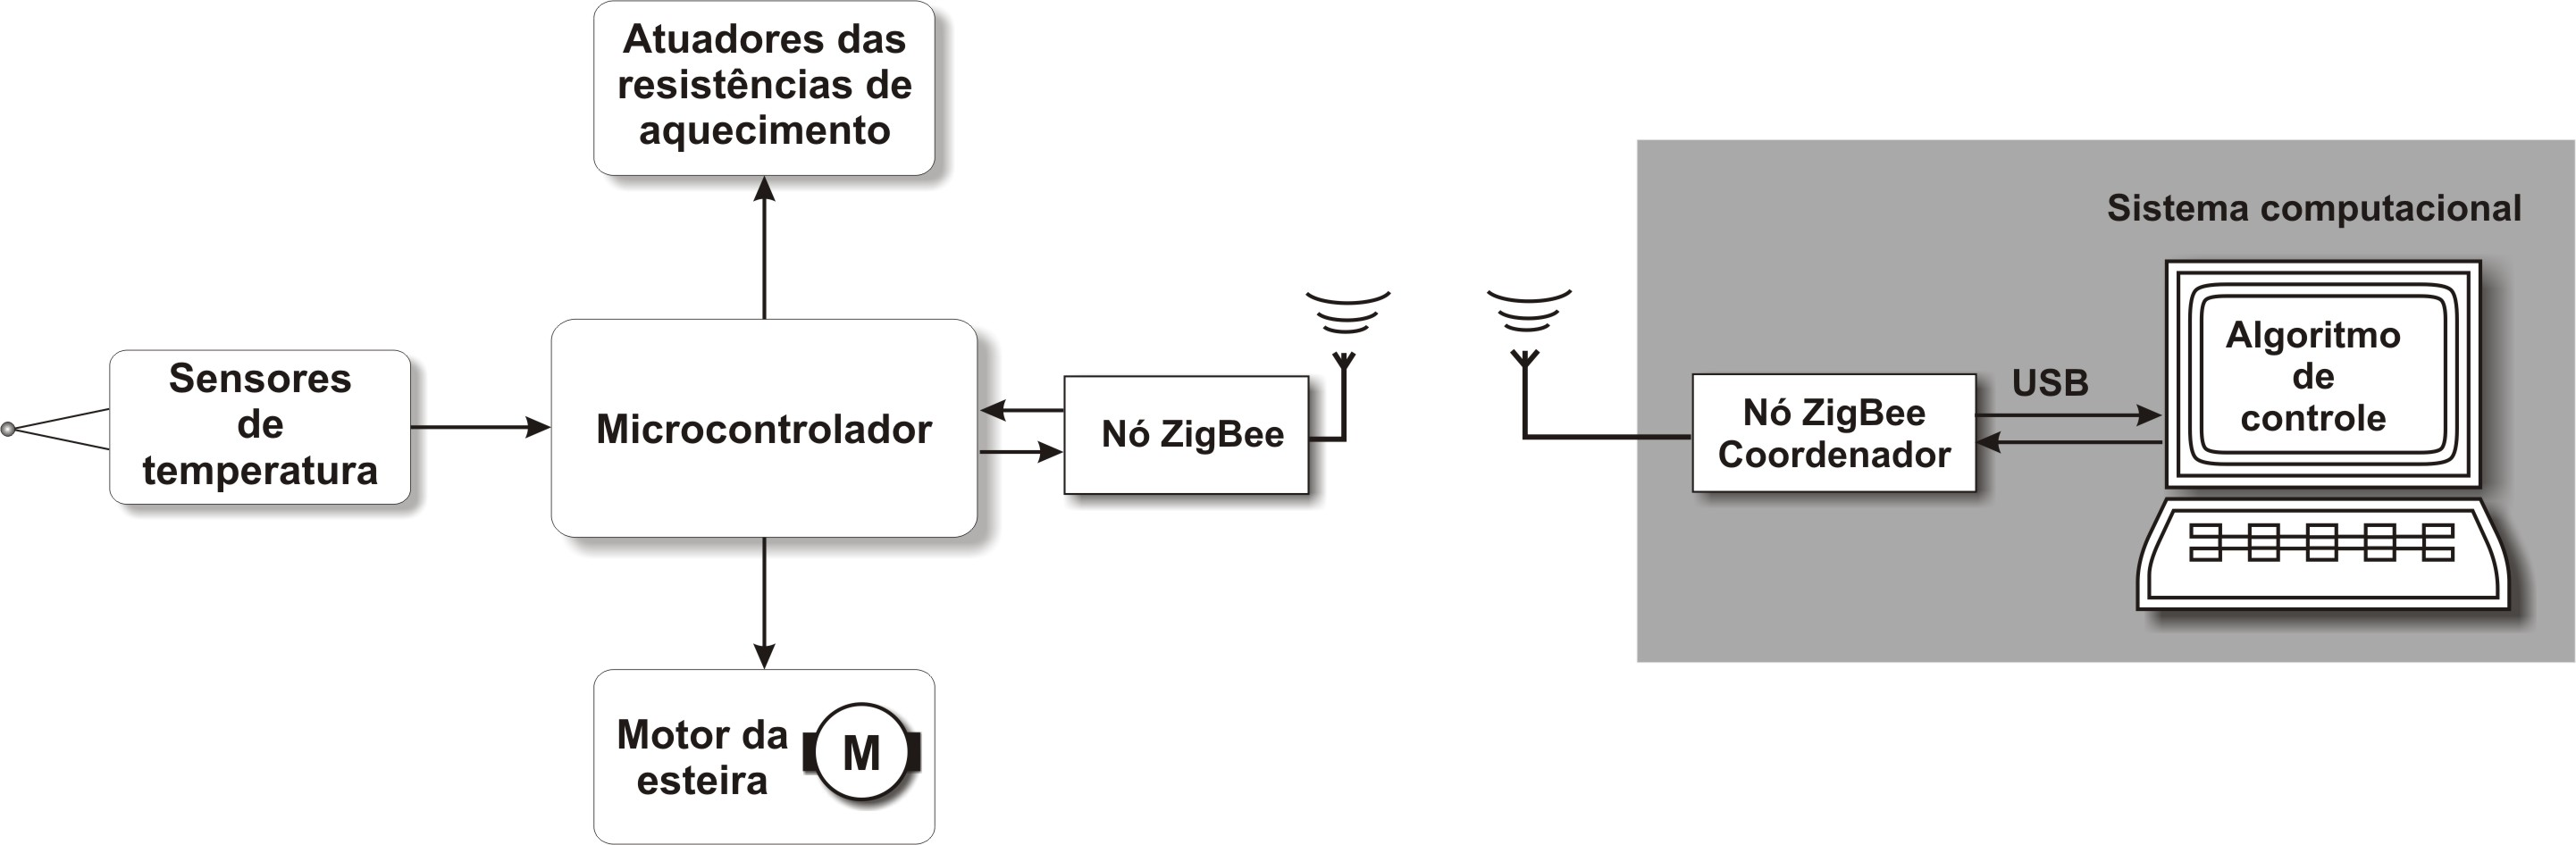
\includegraphics[width=\textwidth]{Figuras/controle_forno}
\caption{Diagrama dos módulos de controle.}
\label{fig:controle_forno}
\end{figure}
 
\subsection{Reconhecimento de Imagem}
 
Foi desenvolvido um software em Python2.7 (anexo \ref{alg:camera}, câmera), que controla uma câmera Raspicam de 5.0 MP (figura \ref{fig:raspicam}). Este software capta imagens a cada 5 segundos por intermédio de comandos na shell do sistema operacional. As imagens são então salvas e uma segunda rotina (anexo \ref{alg:camera}, reconhecimento) é chamada para analisar a mesma.

\begin{figure}[H]
\centering
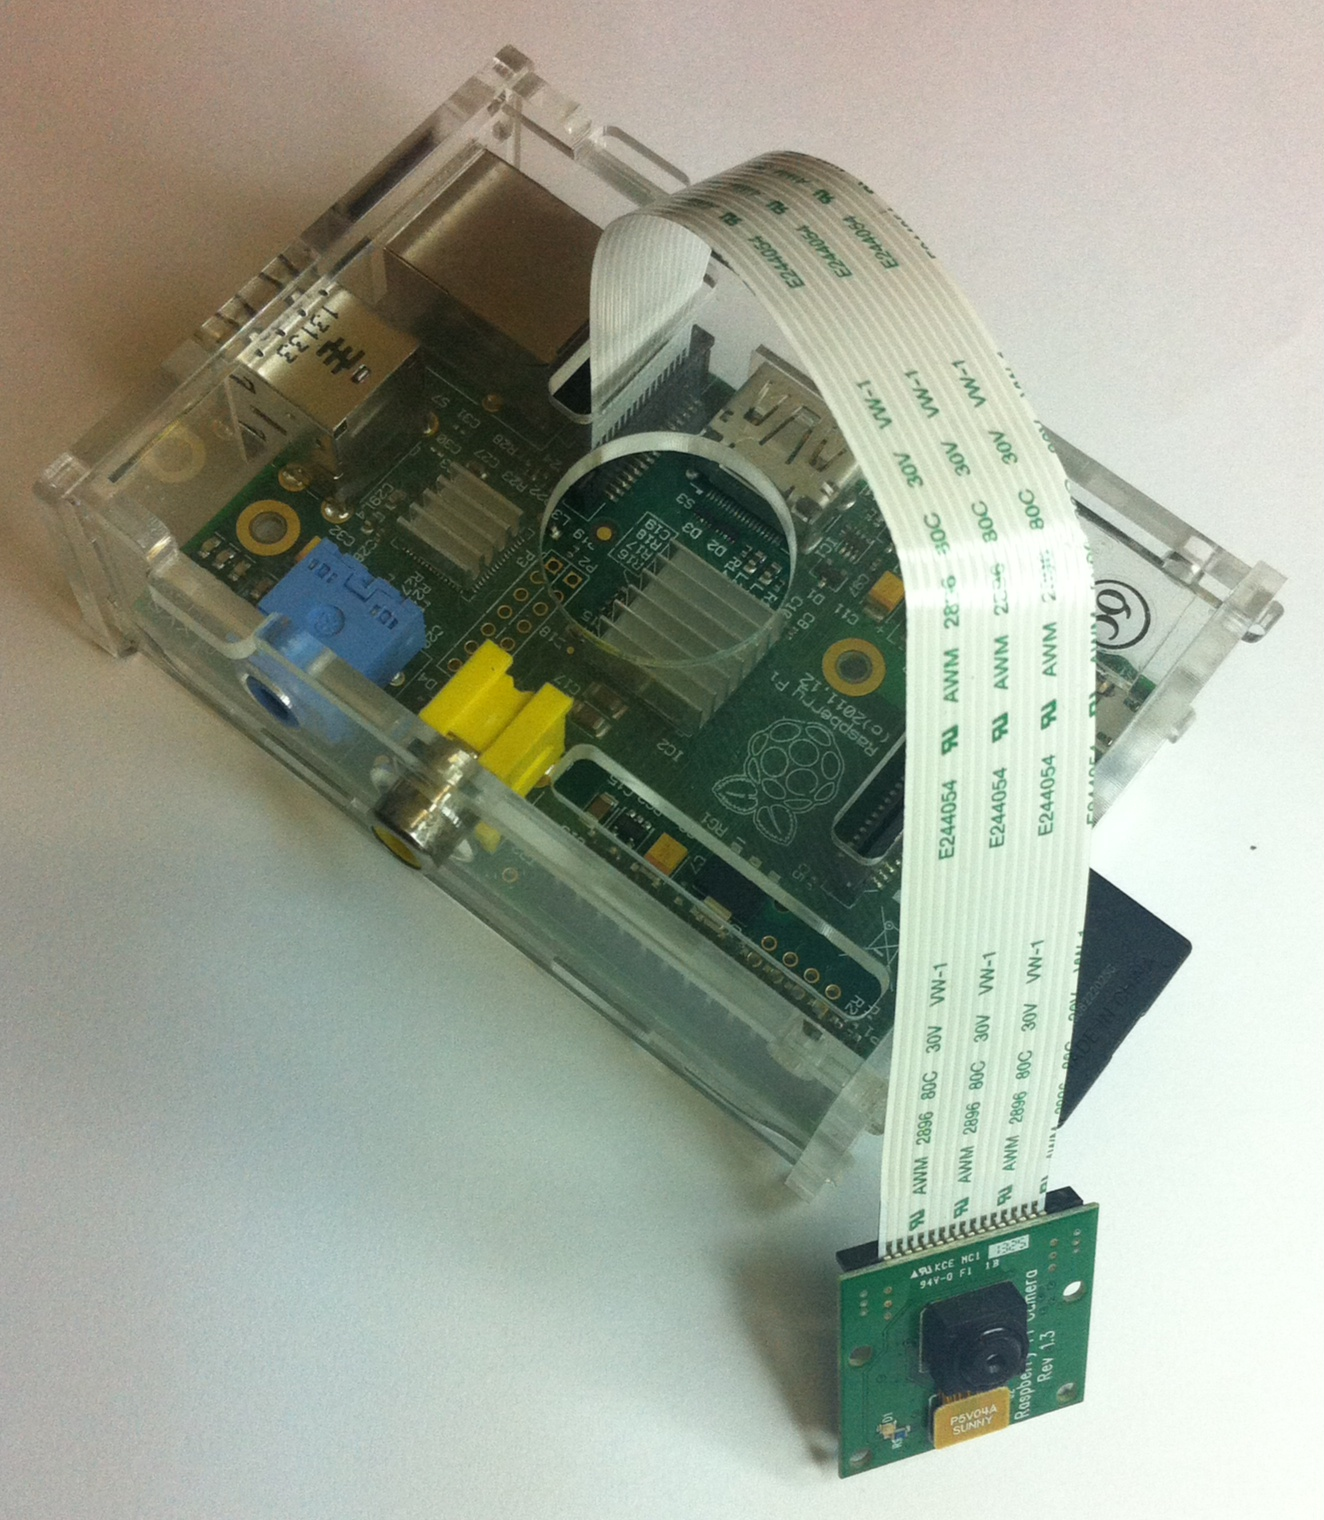
\includegraphics[width=\textwidth]{Figuras/raspicam}
\caption{Raspberry Pi com módulo câmera Raspicam 5 MP para Raspberry Pi}
\label{fig:raspicam}
\end{figure}

Este segundo script também foi desenvolvido em Python2.7 e conta com o auxílio da biblioteca de visão computacional OpenCV. Neste script, a imagem salva é tratada e analisada, retornando a quantidade de biscoitos ou bolachas que estão na entrada da esteira do forno. 

Este script possibilita que o processo de assamento seja iniciado automaticamente quando o produto chega na entrada da esteira. Outra utilidade é uma estimativa da massa total a ser assada, já que o programa retorna a área superior do alimento e a espessura é, em geral, padronizada. 

\subsection{Controle PID}

Foi escrito um algoritmo genérico de controle PID, em Python2.7, com uma classe PID que pode ser instanciada e utilizada pelo sistema de controle. 

Futuramente serão feitos experimentos para se encontrar os melhores parâmetros $K_p$, $K_i$ e $K_d$ e o controle será integrado ao sistema geral de controle

\subsection{Software de Controle - Interface Gráfica}
 
A interface gráfica foi feita utilizando a biblioteca PyQt4, que é uma extensão do Framework Qt para Python2.7. O design da interface foi feito utilizando o software QtDesigner e o resultado foi compilado utilizando o utilitário de linha de comando pyuic4.

Para que o sistema fique modular, o controle da interface foi feito em um script separado, que importa a classe da interface gráfica compilada. 

O software integra um modo manual além do modo de controle automático, permitindo que o usuário possa pausar ou alterar o processo se desejado. Pela interface, o usuário tem informação sobre a câmera na entrada do forno, quantidade de biscoitos, valor da temperatura nos sensores, a simulação térmica e também os controles manuais do forno.





    \chapter{Resultados Parciais e Discussões}\label{resultados}

\section{Simulação da Temperatura}

\subsection{Simulação do perfil térmico em 1D}

A equação \ref{eq:simplificada} foi resolvida analiticamente com os parâmetros descritos em \ref{teste_alg} e a solução encontrada é dada pela equação \ref{eq:sol_1d}.

\begin{equation}\label{eq:sol_1d}
T(x) = 120+(100 \cdot e - 60) \cdot x-(100 \cdot e^x)
\end{equation}

Este resultado é mostrado na figura \ref{fig:dif_fin_1d}, onde ele é comparado com vários métodos para resolução das equações de diferenças finitas. Nele, o espaço (de 0 a 1m) foi discretizado em 100 pontos e os métodos iterativos utilizaram 2000 iterações. 

\begin{figure}[H]
\centering
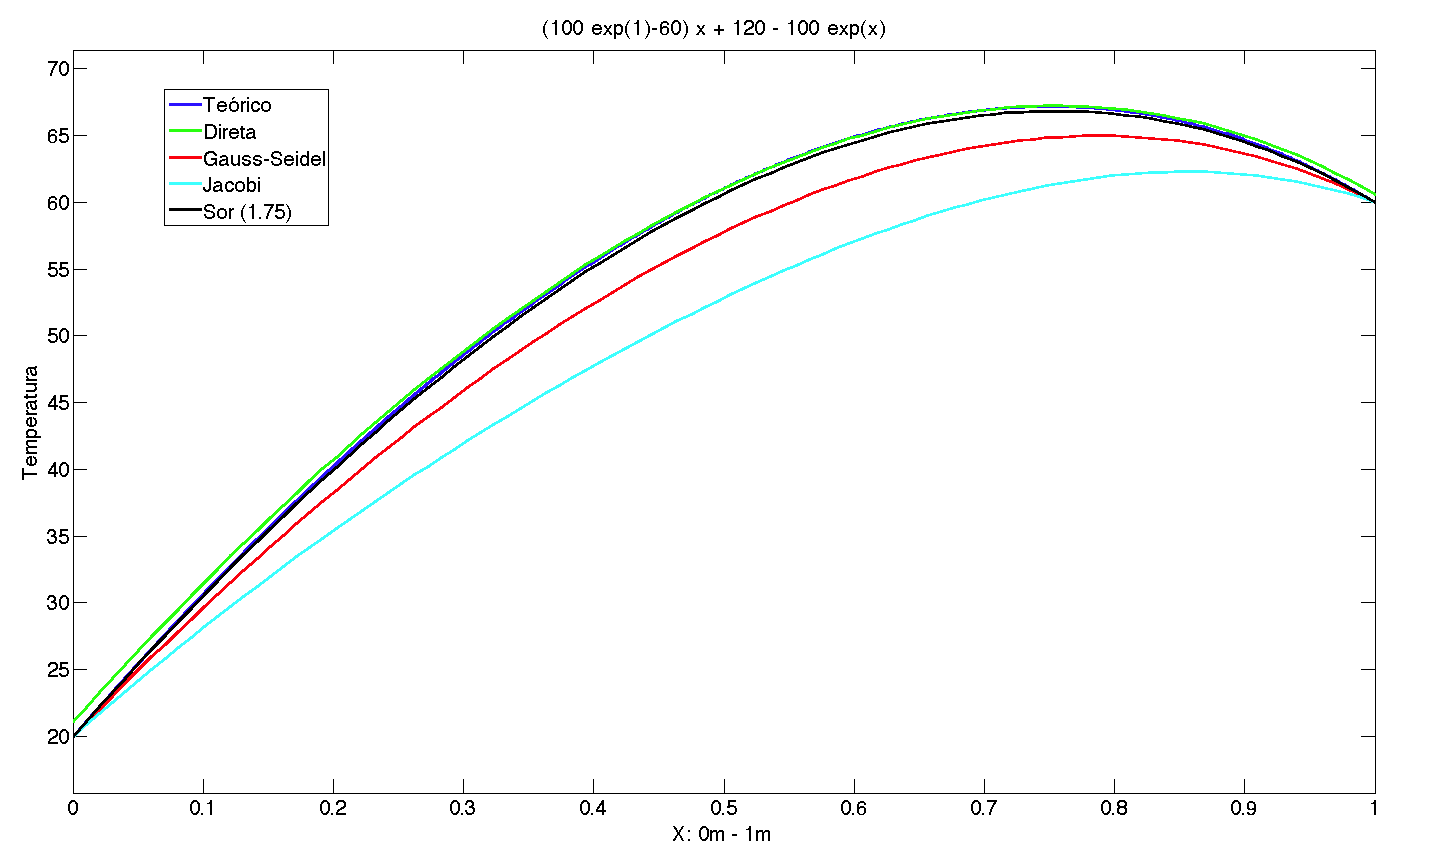
\includegraphics[width=\textwidth]{Figuras/dif_fin_1d}
\caption{Vários Algoritmos de Diferenças finitas em 1d}
\label{fig:dif_fin_1d}
\end{figure}
Como pode ser observado na figura \ref{fig:dif_fin_1d}, os métodos direto e SOR tiveram o melhor resultado, se aproximando da solução analítica. Com mais iterações todos os métodos iterativo convergem porém o método de Jacobi foi é o que necessita de mais iterações, seguido pelo método de Gauss-Seidel e o SOR foi o método iterativo que apresentou melhor resultado. 

Também foi testado o tempo necessário para a convergência dos vários métodos. Como os métodos iterativos convergem assintóticamente, foi estabelecido um erro limite para testar a quantidade de iterações para convergência. Este erro foi definido como a diferença entre a solução direta e o método direto, para que este também pudesse entrar na comparação de forma justa. 

Os valores para o resultado estão apresentados na tabela \ref{tab:tempo_metodos}. 

\begin{table}[htbp]
    \caption{Tempo de execução e número de iterações necessárias para se resolver o problema da difusão térmica 1D, comparado com solução analítica (erro < 0.001) }
    \label{tab:tempo_metodos}
    \vspace{1em}
    \centering
    \begin{tabular}{l r r r r}
        \toprule
        Método  	        & Tempo (s)             & Tempo Normalizado & Iterações     	\\
        \midrule
        Direto   	        & $6,44 \cdot 10^{-4}$  & 1,058	            & - 		        \\
        Jacobi	            & $1,85 \cdot 10^{-1}$  & 302,1             & 12475             \\
        Gauss-Seidel   	    & $3,82 \cdot 10^{-2}$	& 62,73		        &  6240		        \\
        SOR            	    & $6,09 \cdot 10^{-4}$	& 1,000		        &    76		        \\
        \bottomrule
    \end{tabular}
\end{table}

Com este resultado, observamos que o método SOR e o método direto foram os mais eficientes em resolver o problema. O método SOR foi o escolhido como o melhor candidato a ser utilizado na simulação devido a escalabilidade para sistemas 2D e 3D, onde resolver a matriz dos coeficientes (equação \ref{eq:matricial}) demanda um tempo que cresce exponencialmente em relação ao tamanho da matriz.  

\subsection{Parâmetro $w$ no método SOR}

Para determinar o melhor parâmetro $w$ do método SOR, o algoritmo foi executado até que se atingisse um erro fixo entre a solução analítica (anexo \ref{alg:sor}. Então, o algoritmo foi executado consecutivamente para valores de $w$ entre 1 e 1,99, com passo de 0,05. Uma contagem do número de iterações necessárias para a convergência foi feita em função de w e o resultado é apresentado na figura \ref{fig:parametro_sor}. O melhor valor de $w$, para o qual a convergência é mais rápida, foi o valor de 1,965.

\begin{figure}[H]
\centering
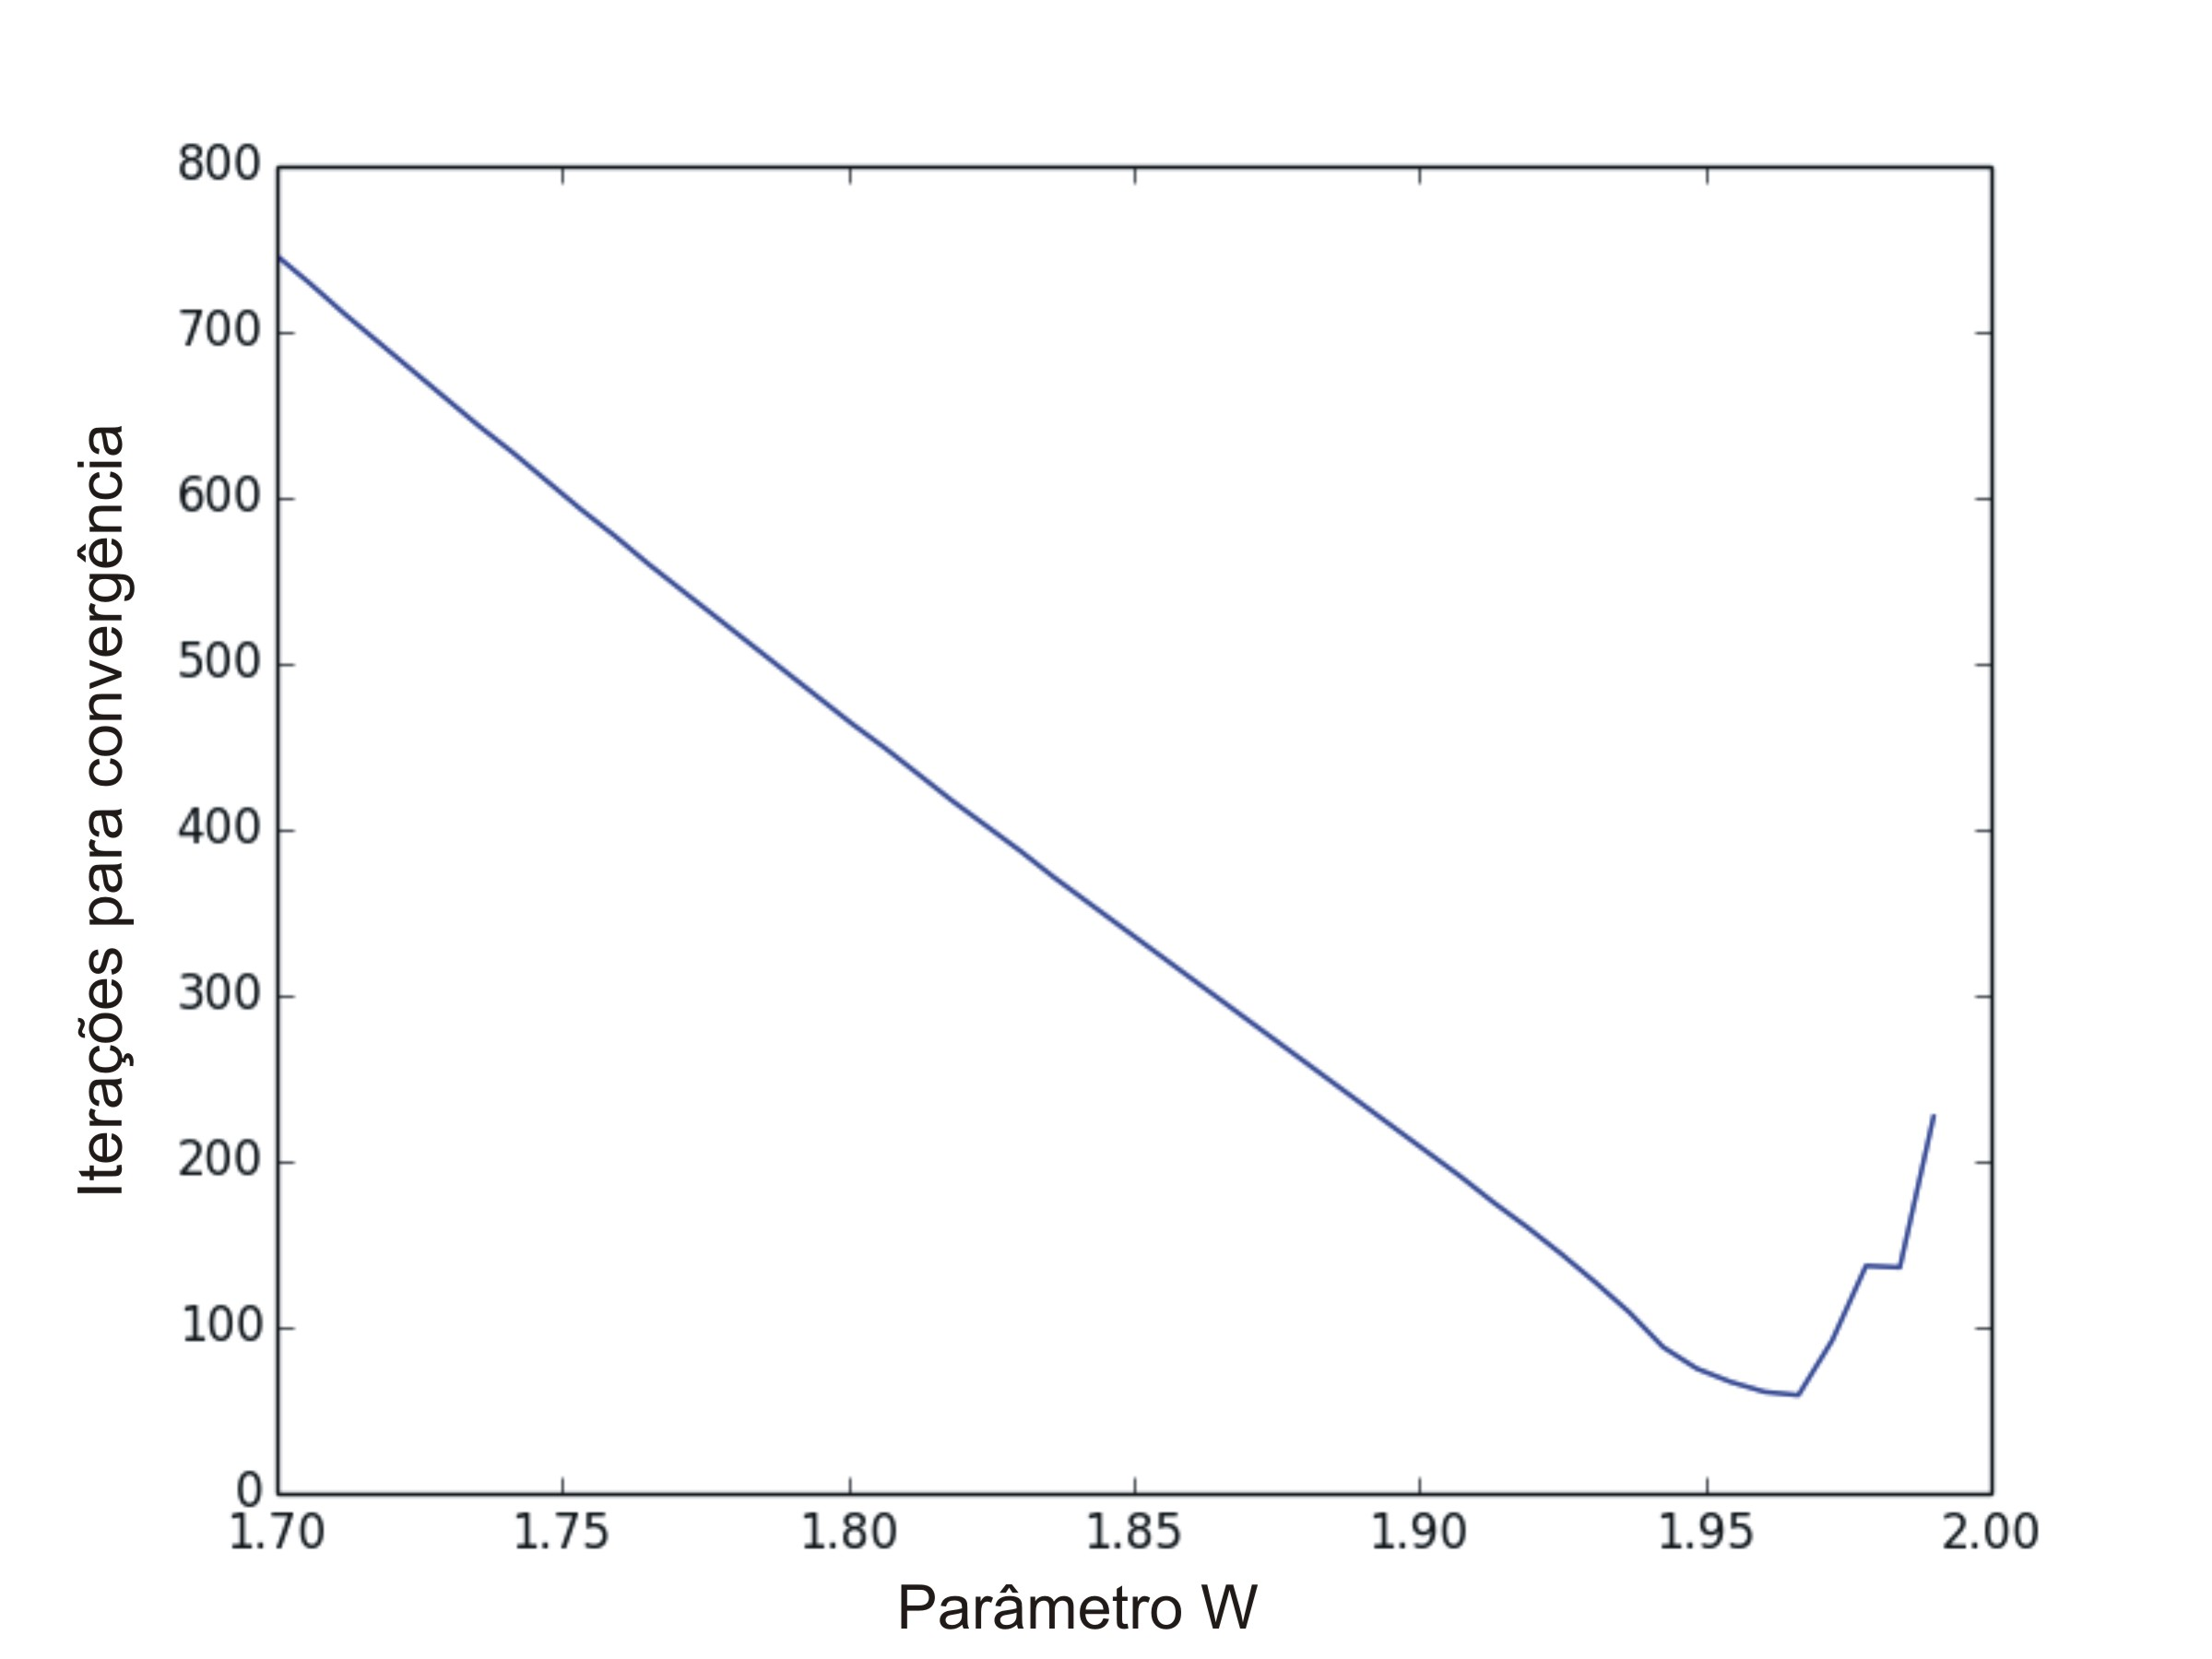
\includegraphics[width=\textwidth]{Figuras/parametro_sor}
\caption{Algoritmo SOR: Número de iterações em função de $w$}
\label{fig:parametro_sor}
\end{figure}

\subsection{Eficiência computacional do algoritmo em várias linguagens}

Para comparar a eficiência computacional do mesmo algoritmo em várias linguagens foi escolhido o método SOR e as linguagens escolhidas foram C/C++, Fortran, Python, Matlab e Octave. Os códigos respectivos encontram-se no anexo \ref{alg:linguagens}, sendo que o mesmo código foi utilizado para o matlab e para o octave, já que a sintaxe é a mesma. Os resultados estão apresentados na tabela \ref{tab:tempo_sor}

\begin{table}[htbp]
    \caption{Tempo de execução do Código de Diferenças Finitas 1D - SOR em várias linguagens}
    \label{tab:tempo_sor}
    \vspace{1em}
    \centering
    \begin{tabular}{l r r r r}
        \toprule
        Linguagem	        & Tempo (s)     & Tempo Normalizado & Desvio Padrão	    \\
        \midrule
        C/C++   	        & 0,007168		& 1,000	            & $9,707 \cdot 10^{-6}$	\\
        Fortran	            & 0,007184      & 1,0023            & $9,797 \cdot 10^{-6}$ \\
        Python/Numpy   	    & 0,070621		& 9,8528		    & $5,997 \cdot 10^{-4}$	\\
        Python-loop   	    & 1,506437		& 210,17		    & $6,73 \cdot 10^{-2}$		    \\
        Matlab-loop   	    & 0,064592		& 9,0116		    & $8,114 \cdot 10^{-4}$	\\
        Matlab-vetorizado   & 0,044488	    & 6,2067		    & $3,197 \cdot 10^{-3}$  \\
        Octave-loop   	    & 7,710252	    & 1075,7		    & $8,3 \cdot 10^{-2}$		    \\
        Octave-vetorizado   & 0,173330		& 24,182		    & $9,48 \cdot 10e^{-4}$ \\
        \bottomrule
    \end{tabular}
\end{table}

As linguagens C/C++ e Fortran foram as que obtiveram melhores resultados, como já era esperado, pois se tratam de linguagens compiladas altamente otimizadas para performance. Nas linguagens interpretadas, notamos uma diferença significativa entre os algoritmos vetorizados e não vetorizados, uma vez a vetorização, tanto no matlab, quanto no octave e no numpy, utilizam rotinas em C (Matlab e Octave) ou Fortran (numpy).

Ambas as linguagens compiladas se mostraram satisfatórias para a execução da simulação, com tempo de execução muito abaixo da ordem de grandeza do tempo de resposta do forno. No entanto, testes em sistemas embarcados ainda devem ser feitos para se averiguar a queda de performance.

\subsection{Eficiência computacional do algoritmo em vários sistemas embarcados}

Nesta etapa, será comparado o mesmo algoritmo em uma linguagem escolhida em vários sistemas embarcados para que se possa escolher o sistema mais adequado. Caso o tempo de simulação esteja muito abaixo do tempo necessário pelo controle PID, será escolhido o hardware que possua mais benefícios em termos de compatibilidade, usabilidade e preço.

\section{Controle}

\subsection{Reconhecimento de Imagem}

Os testes iniciais mostram que o algoritmo utilizado foi capaz de captar os objetos de acordo com o formato e a cor, não gerando falsos positivos e errando apenas quando o alimento não estava no padrão que deveria figura \ref{fig:opencv}.  

Para o filtro de cores, o melhor resultado foi obtido realizando uma transformada do espectro RGB para HSV, garantindo que seja buscada apenas um range específico de cor e que o brilho e iluminação não interferissem no resultado.  

\begin{figure}[htbp]
    \centering
    \subfloat[Entrada]{\label{fig:Entrada}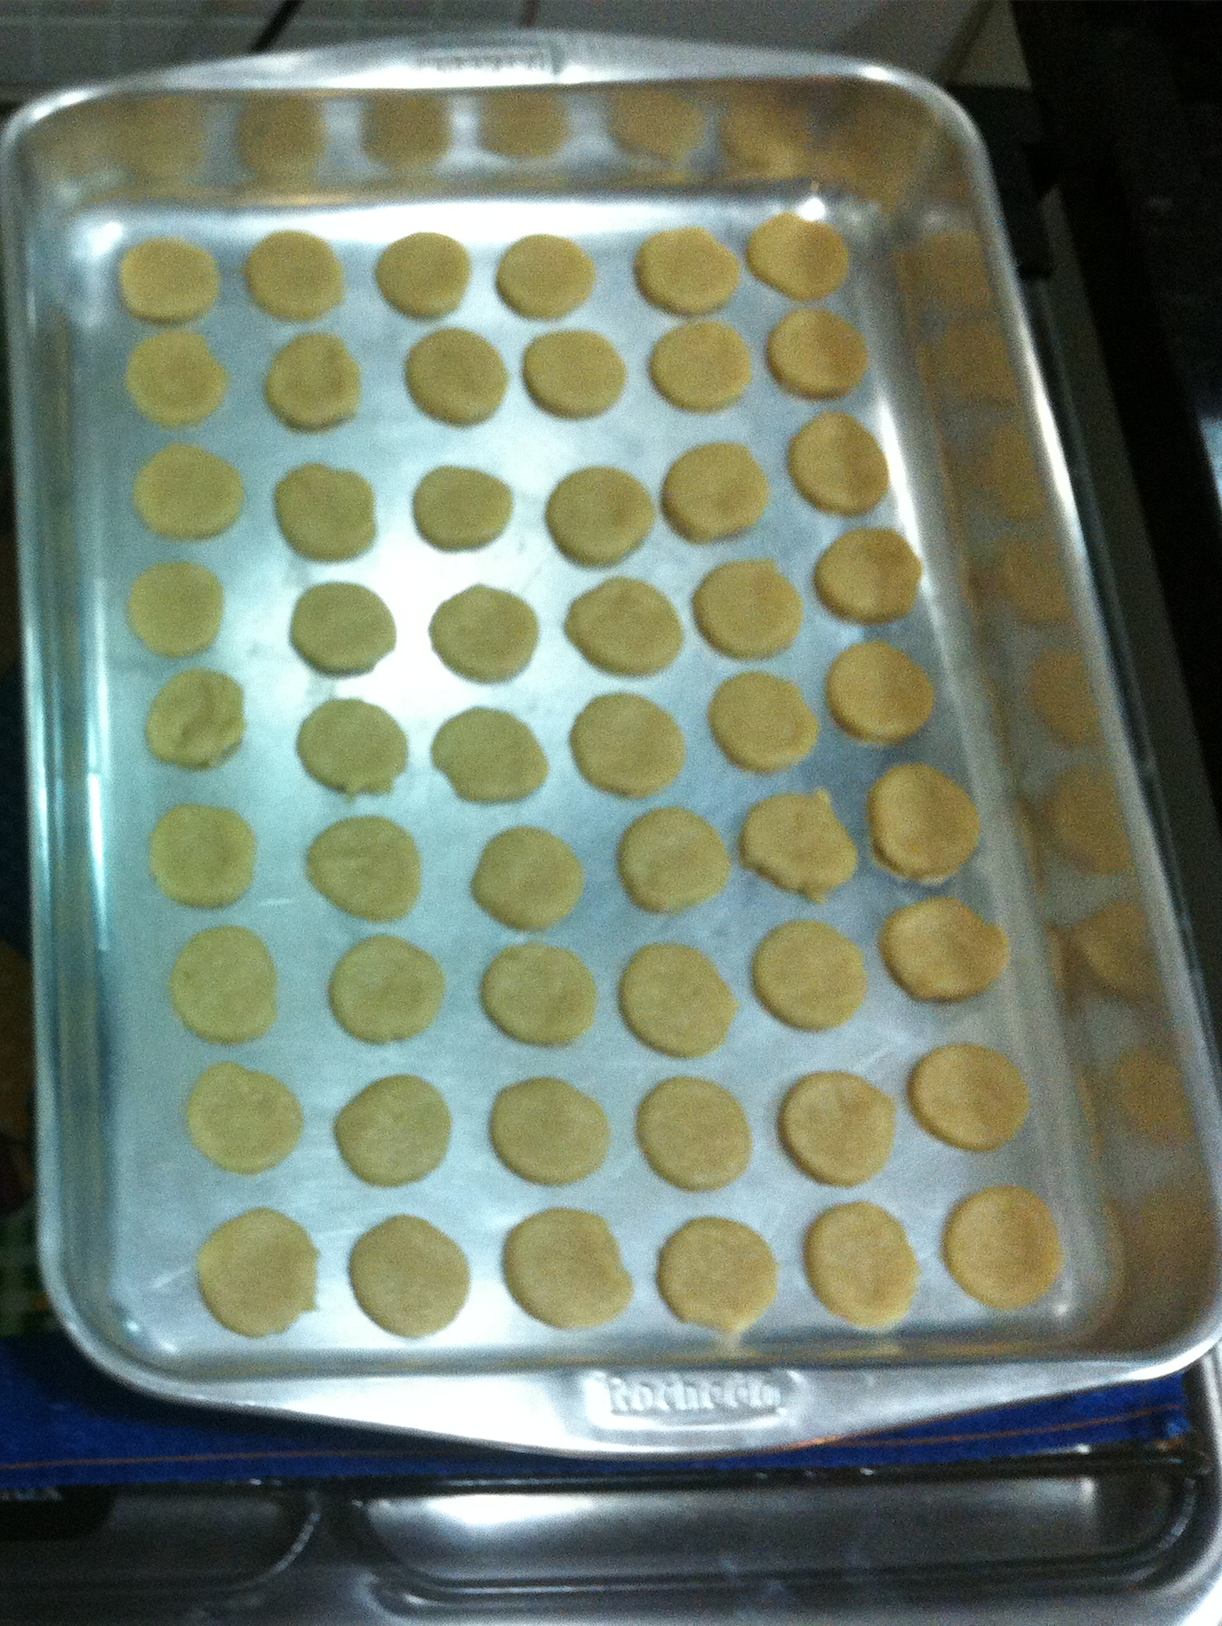
\includegraphics[width=200pt]{Figuras/imagens_biscoito/antes}}\vspace{11pt}
    \subfloat[Filtro Limiar Adaptativo]{\label{fig:filtro_limiar}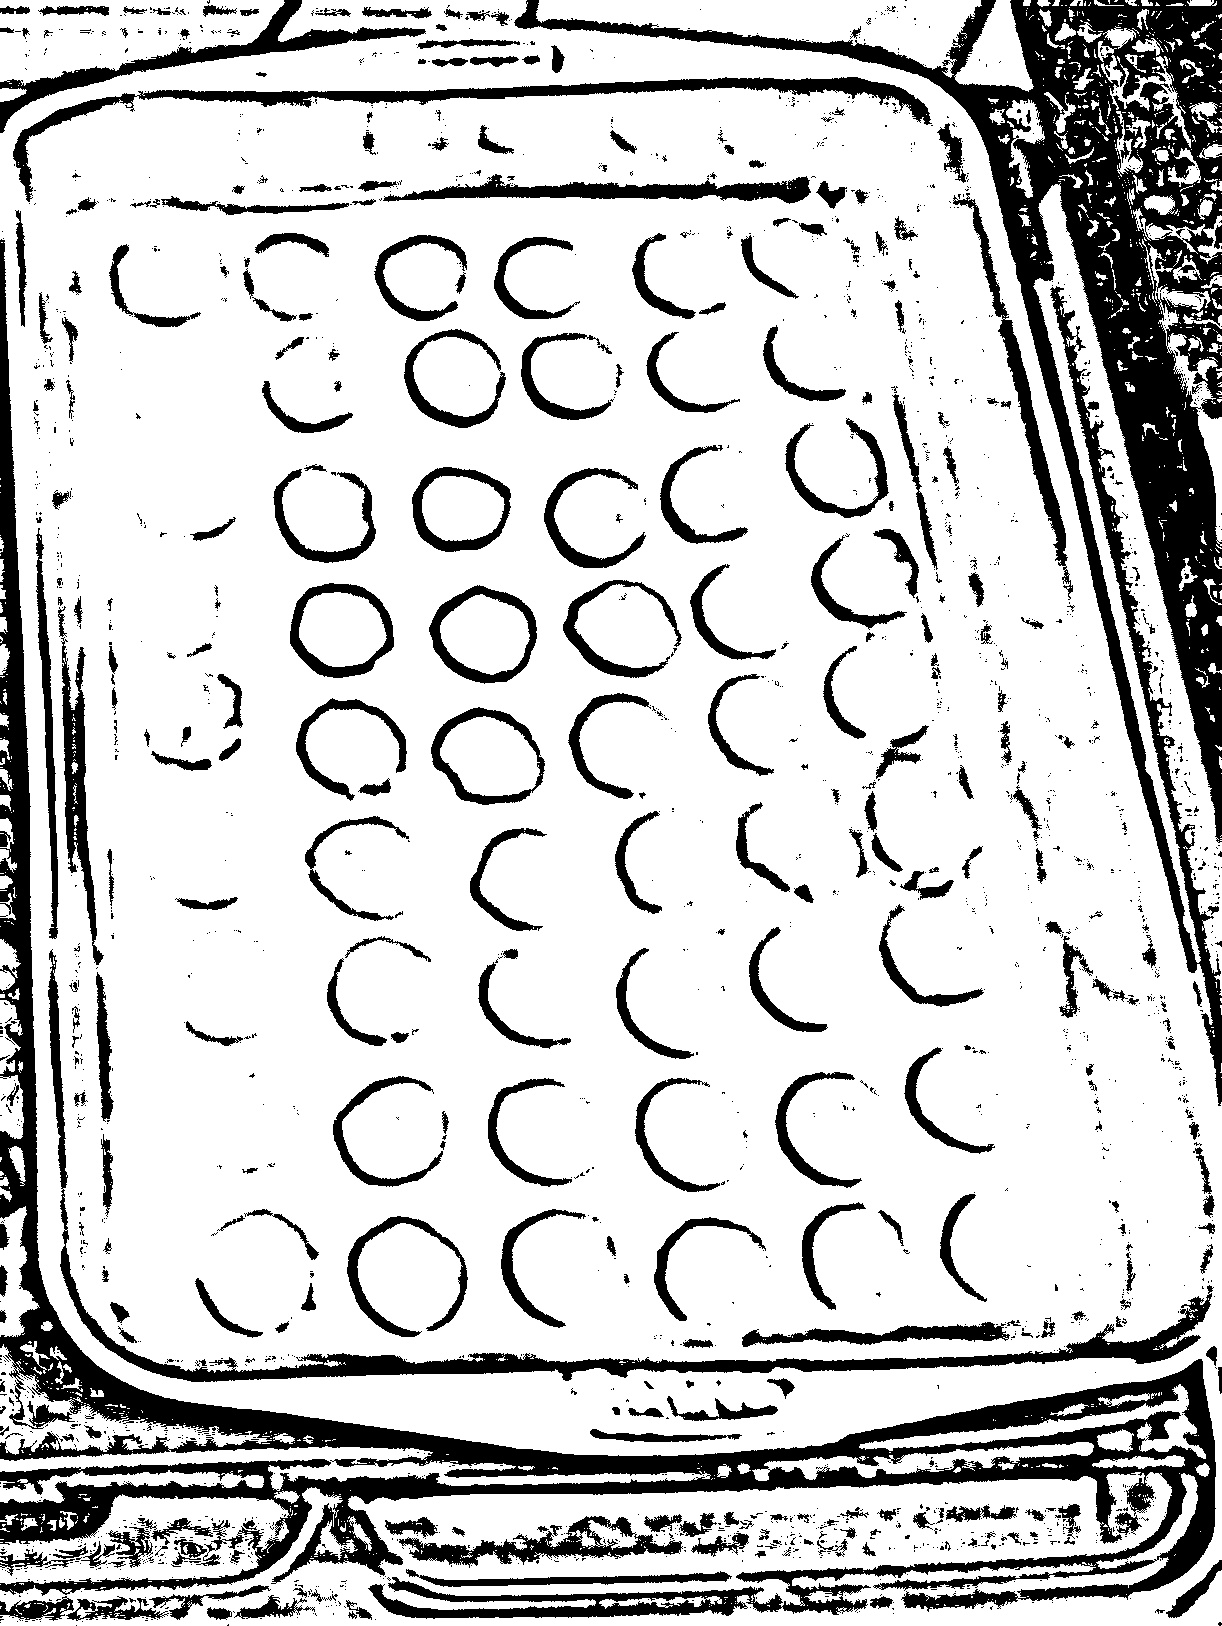
\includegraphics[width=200pt]{Figuras/imagens_biscoito/biscoito_limiar}}\\
    \vspace{-18pt}
    \subfloat[Filtro HSV]{\label{fig:filtro_hsv}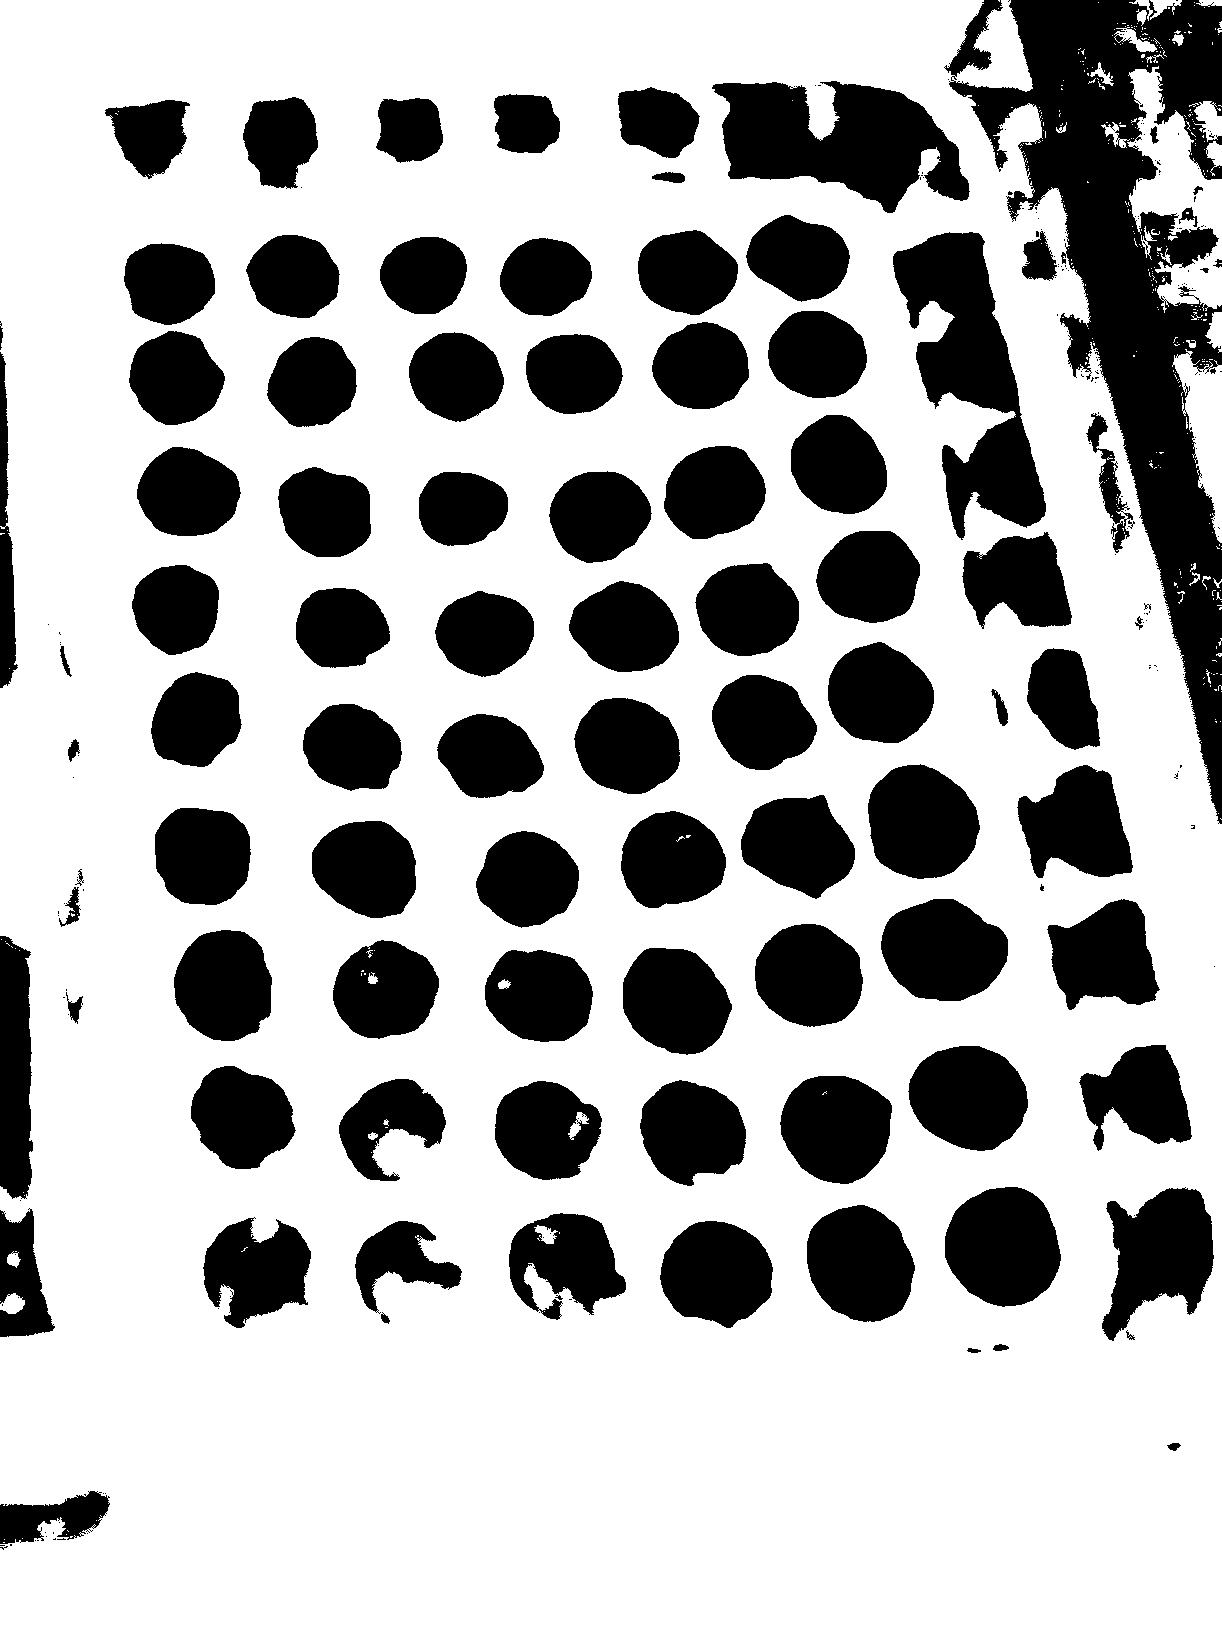
\includegraphics[width=200pt]{Figuras/imagens_biscoito/biscoito_filtro_cor}}\vspace{11pt}
    \subfloat[Objetos redondos reconhecidos]{\label{fig:redondo}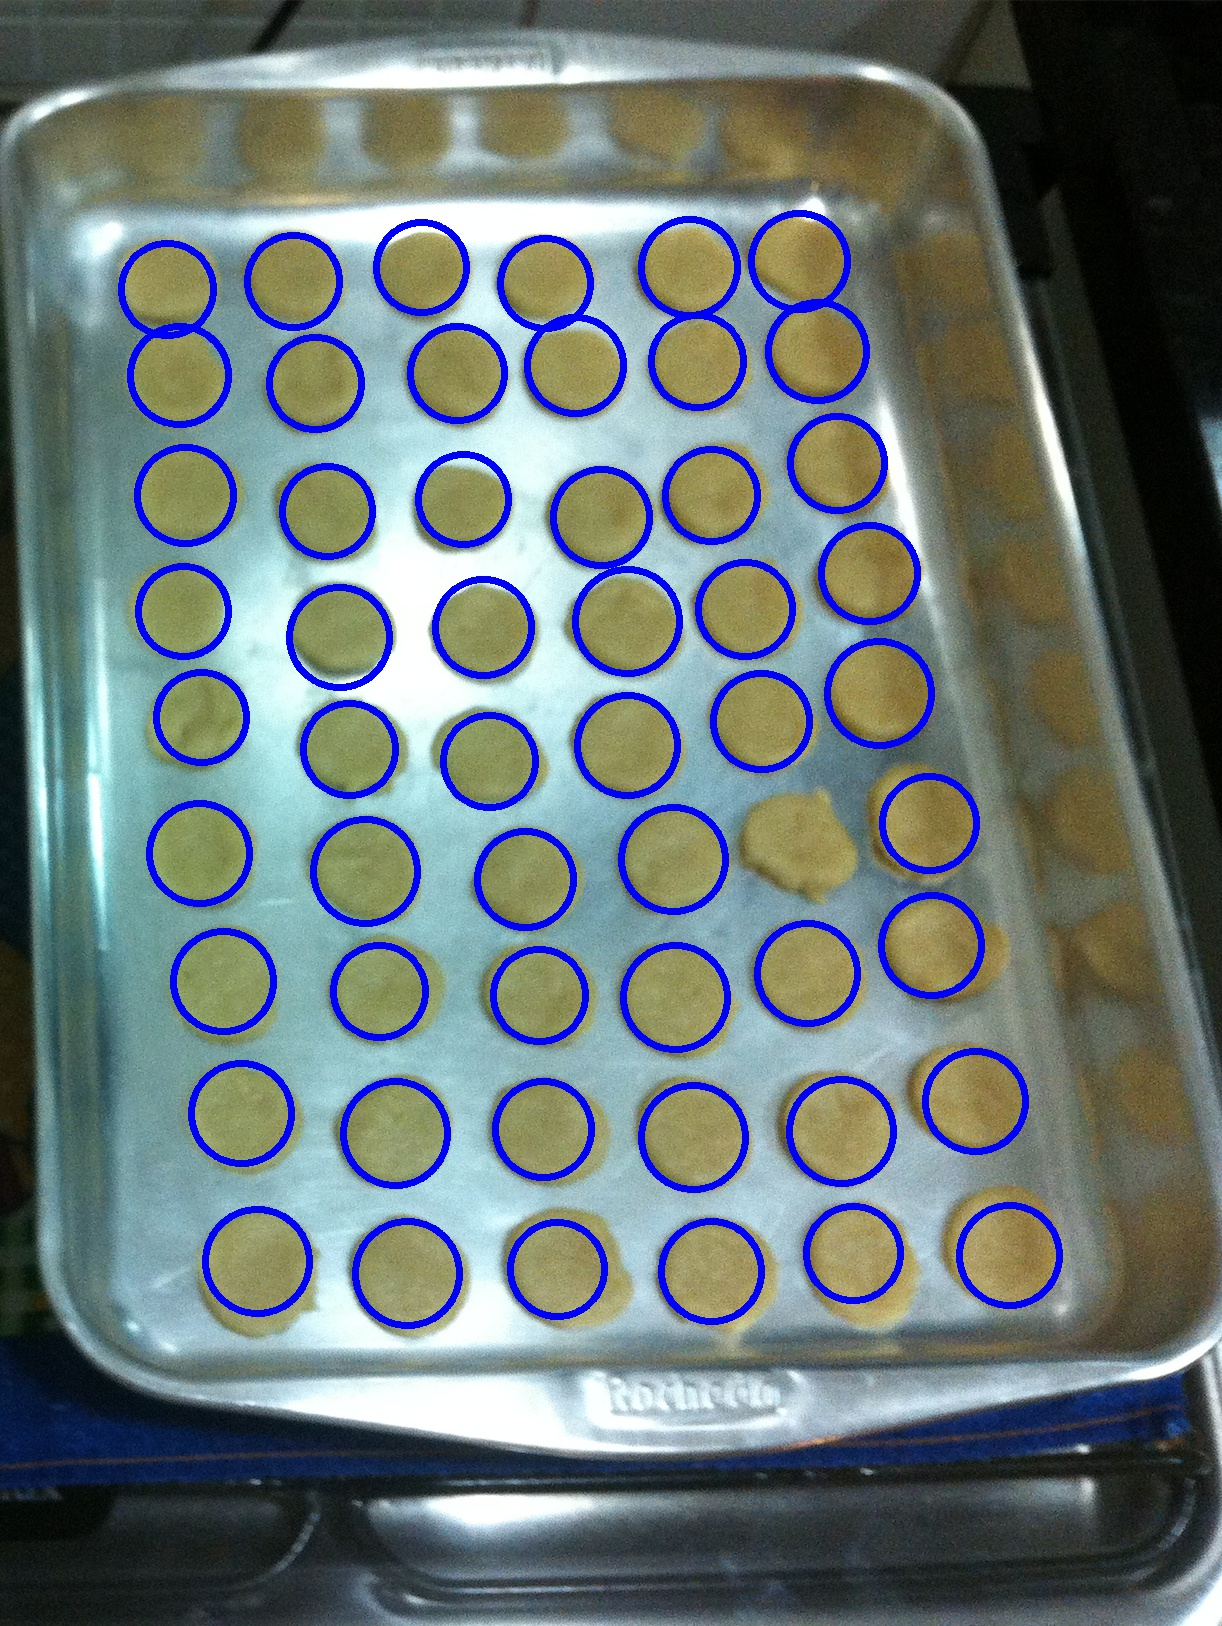
\includegraphics[width=200pt]{Figuras/imagens_biscoito/biscoito_reconhecido}}
    \caption{Processamento da imagem, iniciando com a imagem pura (a), aplicação de filtros limiar adaptativo (b), filtro HSV (c) e por último o reconhecimento dos objetos redondos na imagem tratada (d)}
    \label{fig:opencv}
\end{figure}

Após a aplicação do filtro de cores, foi aplicado um limiar binário, para preparar a imagem para o reconhecimento de formatos (no caso do teste, de objetos redondos). O limiar utilizado foi o adaptativo com filtro gaussiano (anexo \ref{alg:camera}, de modo que não dependesse de um limiar fixo, que pode alterar a detecção caso as condições de claridade sejam alterados.

Os resultados foram satisfatórios na detecção de biscoitos redondos e futuros testes utilizando as informações da área e quantidade de biscoitos reconhecidos será feita para estivar a massa total que entrará no forno. Estes dados poderão ser inseridos no algoritmo de controle caso a massa seja um parâmetro que possa alterar o perfil de temperatura.

Um fator importante da coleta de imagem é o controle de qualidade, possibilitando que o sistema possa ser alterado para controlar a qualidade do produto produzido. 

\subsection{Software de Controle - Interface gráfica}

Na figura \ref{fig:gui_control} vemos o resultado da interface gráfica produzida. Ela permite o controle automático e manual do forno, mas a integração de todos os códigos de simulação ao controle automático ainda não foram realizados devido a necessidade de testes do controle PID. 

Testes qualitativos mostraram indicam que a interface funcionou corretamente mas testes futuros ainda deverão ser feitos. Uma outra possibilidade que será analisada é a utilização de uma interface gráfica via web, diminuindo a necessidade de uso da memória para processamento gráfico, uma vez que isto será feito do lado do “cliente” e não do servidor. 

\begin{figure}[H]
\centering
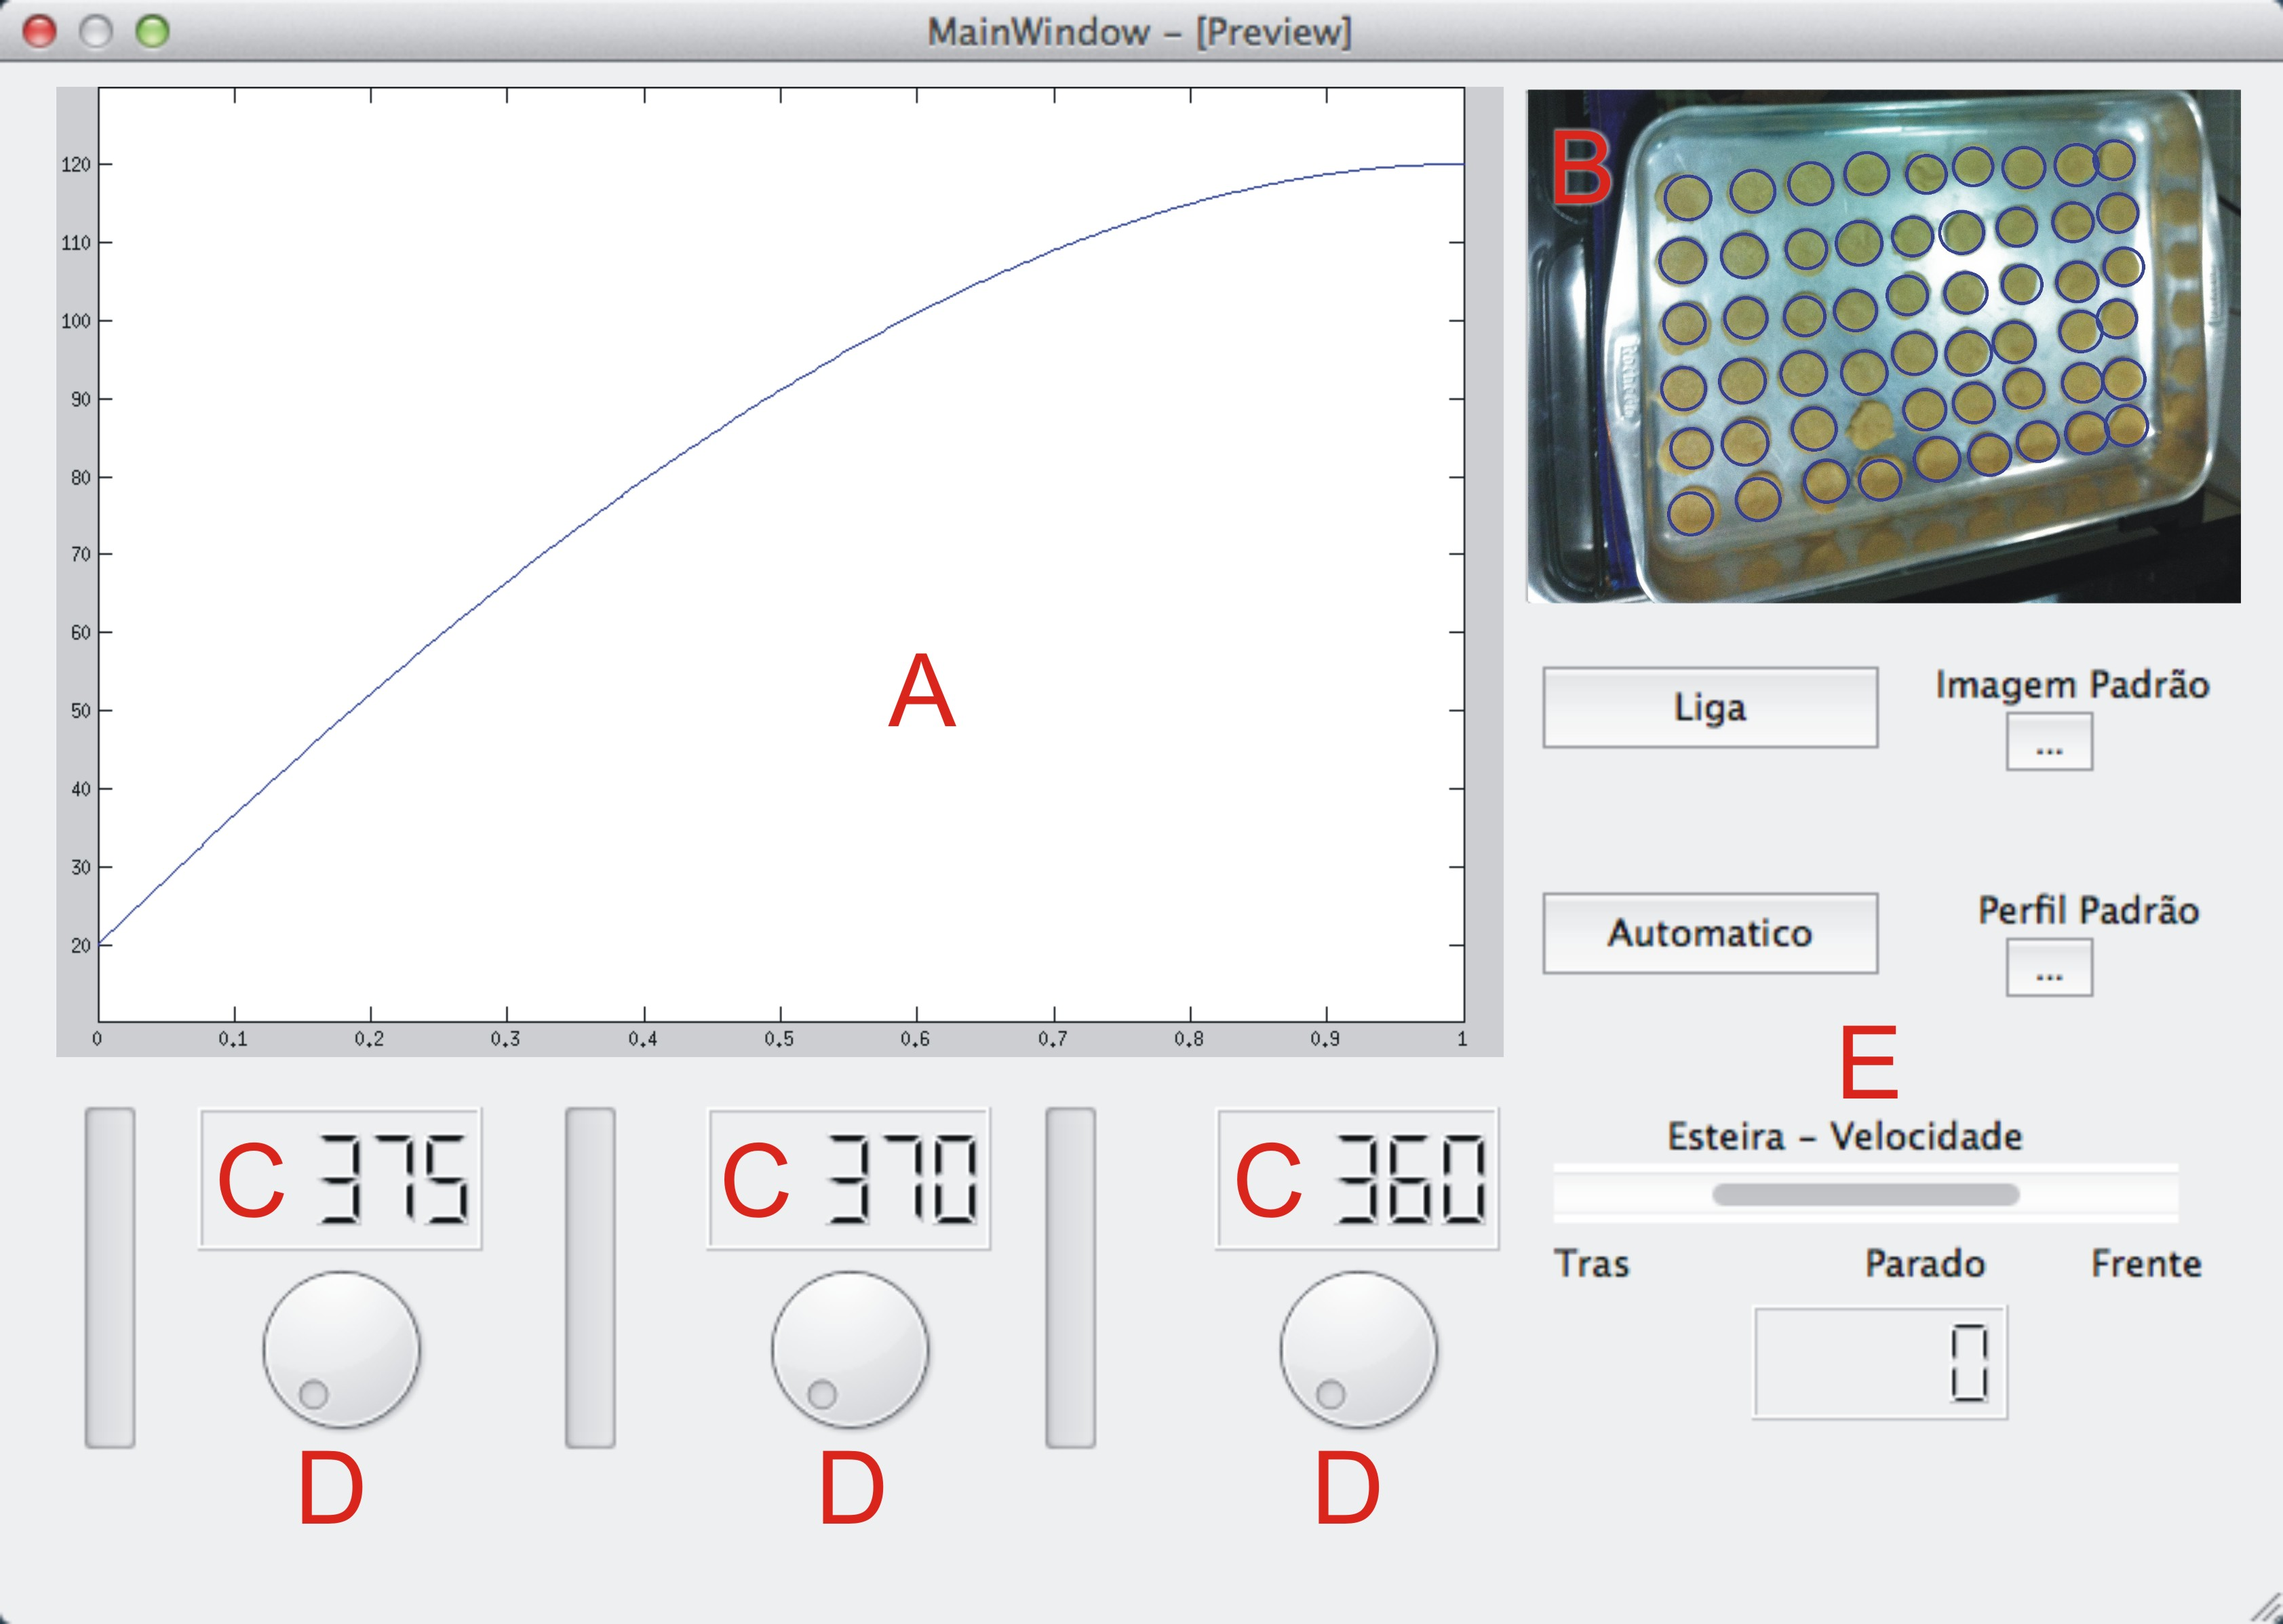
\includegraphics[width=\textwidth]{Figuras/gui_control2}
\caption{Software de controle. A: Resultado da simulação térmica ao longo do perfil do forno. B: Imagem da Câmera na entrada do forno com reconhecimento de padrão. C: Leitura do sensor de temperatura nas três zonas térmicas. D: Controle manual a potência nas três zonas térmicas. E: Controle manual da velocidade da esteira.}
\label{fig:gui_control}
\end{figure}























    \chapter{Conclusões Parciais}\label{conclusao}

Os testes de simulação foram satisfatórios porém comparação com resultados experimentais ainda é necessária para validar o procedimento. Caso os resultados experimentais discordem da simulação, novos parâmetros deverão entrar no modelo matemático do problema, como o fluxo de ar e o metal da esteira no interior do forno.  

Com a simulação satisfatória, serão feitos experimentos para se encontrar o controle otimizado do forno e então novos testes de perfil serão realizados.
    % Pós-Texto
    \bibliographystyle{abnt2}
    %\bibliographystyle{apa}%{apalike}  % Formato da bibliografia
    \bibliography{referencia.bib}    % Arquivo .bib
    \chapter{Apêndice}\label{apêndice}

\section{Diferenças Finitas 1D - Vários métodos}\label{alg:dif1d}

Programa que implementa a solução da equação de difusão de calor em 1 Dimensão utilizando os métodos Direto, Jacobi, Gauss-Seidel, e SOR, utilizando uma condição de contorno que permite encontrar a solução analítica para fins de conparação. Programa implementado em Python2.7

\singlespacing
\lstset{language=Python}
\begin{lstlisting}
from __future__ import division
import numpy as np
import matplotlib.pyplot as plt
import pylab
import time

###################### Funcoes #########################################
def tridiagonal(A,B):
    '''
    Programa que resolve a equacao AX = B, recebendo como entrada
    as matrizes A e B e retornando X.
    Precondicoes: 
    A matriz A deve ser quadrada (n x n)
    A matriz B deve ser uma matriz coluna (n x 1)
    A matriz A deve ser tridiagonal
    '''
    [Alinha,Acoluna] = A.shape
    [Blinha,Bcoluna] = B.shape
    if ( Acoluna !=  Alinha):  # Checa se a matriz A e quadrada
        print ' A Matriz A nao e quadrada'
        return
    if ( Alinha !=  Blinha):# Checa se AxB existe
        print ' A x B nao e uma operacao matricial permitida'
        return
    if ( Bcoluna != 1 ): # Checa se B e uma matriz coluna
        print ' A matriz B nao possui apenas uma coluna'
        return    
    # Checando se a matriz e tridiagonal:
    for i in range(Alinha):           # Checa a parte superior da matriz
        for j in range(i+2,Alinha):
            if ( A[i,j] != 0 ):
                print 'A matriz nao e tridiagonal ' ,  'A[', i , ',' , j , ']'
                return
        for j in range(0,i-2):
            if ( A[i,j] != 0 ):
                print 'A matriz nao e tridiagonal ' , 'A[', i , ',' , j , ']'
                return       
    ## Metodo TDMA
    print ' Todas as condicoes corretas ! '
    x = np.zeros([Alinha,1])
    print A, B
    for i in range(1,Alinha):
        a1 = A[i,i-1]
        a2 = A[i-1,i-1]
        m = a1/a2
        A[i,i] = A[i,i]   - (m*A[i-1,i])
        B[i]   = B[i]     - (m*B[i-1])
    x[Alinha-1] = B[Alinha-1] / A[Alinha-1,Alinha-1]
    
    for k in range(Alinha-2,-1,-1):
        x[k] = ( B[k] - (A[k,k+1]*x[k+1]) )/A[k,k]
    return x

######################## Condicoes do problema #######################
L0 = 0
Lf = 1
n  = 100
deltax  = (Lf - L0)/n
deltax2 = (Lf - L0)/(n+1)  # verificar n+1
x       = np.linspace(L0,Lf,n)
f       = 100*np.exp(x)
T0      = 20
Tf      = 60

####################### Metodo Direto ################################
tic = time.time()
A = np.zeros([n,n])
B = np.zeros([n,1])
B1 = np.zeros([n,1])
B2 = np.zeros([n,1])
B2[0]   = T0
B2[n-1] = Tf

for i in range(n):
    B1[i] = f[i]

B = -(deltax2)*(deltax2)*B1 - B2

for i in range(n):
    for j in range(n):
        if ( j == i - 1 ):
            A[i,j] = 1
        elif ( j == i ):
            A[i,j] = -2
        elif ( j == i + 1 ):
            A[i,j] = 1
        else:
            A[i,j] = 0
print B.size
Y = tridiagonal(A,B)
toc = time.time() - tic
plt.figure(1)
plt.plot(x,Y)
#pylab.show()

###################### Metodos Iterativos ############################

iter = 2000
x = np.linspace(L0,Lf,n)
J = T0 + (Tf-T0)*x
J[0]   = T0
J[n-1] = Tf
J2 = T0 + (Tf-T0)*x
J2[0]   = T0
J2[n-1] = Tf
J3 = T0 + (Tf-T0)*x
J3[0]   = T0
J3[n-1] = Tf

###################### Gauss - Seidel ################################

tic2 = time.time()
for k in range (iter):
    for i in range(1,n-2):
        J[i] = (J[i-1] + J[i+1] + deltax*deltax*f[i])/2
toc2 = time.time() - tic2

###################### Jacobi  ########################################

tic3 = time.time()
for k in range (iter):
    for i in range(1,n-2):
        Jant  = J2
        J2[i] = (J2[i-1] + J2[i+1] + deltax*deltax*f[i])/2
toc3 = time.time() - tic3

###################### SOR  ########################################

tic4 = time.time()
for k in range (iter):
    for i in range(1,n-2):
        Jn = (J3[i-1] + J3[i+1] + deltax*deltax*f[i] )/2   
        J3[i] = J3[i] + 1.7*( Jn - J3[i] )
toc4 = time.time() - tic4

#######################  Jacobi - numpy ############################
J4 = T0 + (Tf-T0)*x
J4[0]   = T0
J4[n-1] = Tf
tic5 = time.time()
for k in range (iter):
    J4[1:n-2] = ( J4[0:n-3] + J4[2:n-1] + deltax*deltax*f[1:n-2] )/2
toc5 = time.time() - tic5

print 'Metodo Direto: ' , toc
print 'Gauss Seidel:  ' , toc2
print 'Jacobi:        ' , toc3
print 'SOR:           ' , toc4
print 'Jacobi f2py:   ' , toc5
plt.plot(x,J)
plt.plot(x,J2)
plt.plot(x,J3)
pylab.show()
\end{lstlisting}
\doublespacing
%%%%%%%%%%%%%%%%%%%%%%%%%%%%%%%%%%%%%%%%%%%%%%%%%%%%%%%%%%%%%%%%%%%%%%%%%%%%%%%%%%%%%%%%%%%%%%%%%%%%%%%%%%%%%%%%%%%

\section{Diferenças Finitas - Várias Linguagens}\label{alg:linguagens}

Compara o tempo de execução do mesmo Algoritmo de Diferenças Finitas em várias linguagens (Python, Matlab, Octave, Fortran90 e c). O algoritmo utilizado como teste é o método SOR com 300 iterações.

Fortran:

\singlespacing
\lstset{language=Fortran}
\begin{lstlisting}
! Temperatura 1d - Funcao conhecida - metodo SOR 
! Calculo do tempo de execucao
implicit none
real start, finish, L0, Lf, deltax, T0, Tf, sor, i2, k2, a, Nz2
integer i, Nz, k
parameter (Nz = 100)
real J(0:Nz-1)
real Jn(0:Nz-1)
real u(0:Nz-1)
real x(0:Nz-1)
real f(0:Nz-1)
integer p
do p =1, 20
	call cpu_time(start)
	L0 = 0
	Lf = 1
	T0 = 20
	Tf = 60
	deltax = (Lf - L0)/Nz 
	sor = 1.9

	do i = 0, Nz-1 ! Preenchendo os valores de x ( de 0 a 1 )
		i2 = real(i)
		Nz2= real(Nz)
		x(i) = i2/Nz2
	enddo

	do i = 0, Nz-1 ! Preenchendo os valores do aquecimento f(x)
		a = x(i)
		f(i) = exp(a)*100
	enddo


	do i = 0, Nz-1 ! Preenchendo os valores iniciais de J 
		J(i) = T0 + ( Tf - T0 )*x(i)
	enddo

	do k = 0, 3000 ! Calculo de J (SOR)
		do i = 1, Nz-2
			Jn(i) = ( J(i-1) + J(i+1) + deltax*deltax*f(i))/2
			J(i) = J(i) + sor*( Jn(i) - J(i) )	
		enddo
	enddo

	!open (unit=2,file='arquivo.txt',status='unknown')	
	!do i = 0, Nz-1
	!	write (2,20) J(i)
	!	write (*,*) J(i)
	!enddo
	!20	format(0P,F7.1,2(3X,1P,E10.4))

	call cpu_time(finish)
	print '("Time = ",ES14.7," seconds.")',finish-start
enddo
end 
\end{lstlisting}

C:

\lstset{language=c}
\begin{lstlisting}
/*
Temperatura 1d - Funcao conhecida - metodo SOR
*/

#include <stdio.h>
#include <math.h> 
#include <time.h>

int main(int argc, char** argv)
{
	clock_t begin, end; // Definindo as variaveis doproblema
	double time_spent;
	float start, finish, L0, Lf, deltax, T0, Tf, sor, i2, k2, a, Nz2;
	int i, k, iter, p;
	int Nz = 100;
	float J[Nz], Jn[Nz], u[Nz], x[Nz], f[Nz];
	for (p = 1; p < 21; p++)
	{
		begin = clock();
		L0 = 0;
		Lf = 1;
		T0 = 20;
		Tf = 60;
		deltax = (Lf - L0)/Nz; 
		sor = 1.9;

		for (i=0; i<Nz; i++) // Preenchendo os valores de x ( de 0 a 1 )
		{
			i2   = (float)i;
			Nz2  = (float)Nz;
			x[i] = i2/Nz2;
		}
		for (i=0; i<Nz; i++) // Preenchendo os valores do aquecimento f(x)
		{
			a    = x[i];
			f[i] = exp(a) * 100.0;
		}
		for (i=0; i<Nz; i++) // Preenchendo os valores iniciais de J 
		{
			J[i] = T0 + ( Tf - T0 )*x[i];
		}

		for (iter=0; iter < 3001; iter++)
		{
			for (i=1; i< Nz-1; i++)
			{
				Jn[i] = ( J[i-1] + J[i+1] + deltax*deltax*f[i])/2.0;
				J[i] = J[i] + sor*( Jn[i] - J[i] );
			}
		}
		end = clock();
		time_spent = (double)(end - begin) / CLOCKS_PER_SEC;
		printf(" tempo: %f \n",time_spent);
	}
	/*for (i=0; i<Nz; i++) // Imprimindo o resultado
	{
		printf("T = %f\n",J[i]);
	}*/
}
\end{lstlisting}

Matlab:

\lstset{language=Matlab}
\begin{lstlisting}
%Temperatura 1d - Funcao conhecida - metodo SOR  
%Calculo do tempo de execucao
L0 = 0;   % posicao inicial da barra
Lf = 1;  % posicao final (tamanho) da barra - em metros
n = 100;  % dividindo o problema em 1000 elementos
deltax = (Lf-L0)/n;
%deltax para o metodo direto
deltax2=(Lf-L0)/(n+1);
x = linspace(L0,Lf,n)';
f = 100*exp(x);
T0 = 20;  % temperatura em x=0 (inicio da barra) em kelvin
Tf = 60;  % temperatura em x=Lf (final da barra) em kelvin
J3 = T0 + (Tf-T0)*x;
J3(1) = T0;
J3(n) = Tf;
for p=1:20
	id = tic;
	for k=1:3000
	    for i=2:n-1     
	       Jn   = (J3(i-1) + J3(i+1) + deltax*deltax*f(i))/2;
	       J3(i) = J3(i) + 1.9*(Jn - J3(i));
	    end
	end
	toc(id)
end
\end{lstlisting}

Matlab Vetorizado:

\lstset{language=Matlab}
\begin{lstlisting}
    % parte principal do algoritmo vetorizada
    for k=1:3000
	    for i=2:n-1     
	       Jn   = (J3(i-1) + J3(i+1) + deltax*deltax*f(i))/2;
	       J3(i) = J3(i) + 1.9*(Jn - J3(i));
	    end
    end
	 
\end{lstlisting}

Python:

\lstset{language=Python}
\begin{lstlisting}

# -*- coding: latin-1 -*-
'''  Temperatura 1d - Funcao conhecida - metodo SOR  
Calculo do tempo de execucao
'''  
from __future__ import division
import numpy as np
import matplotlib.pyplot as plt
import pylab
import time

for p in range(1,21):
	tic = time.time()
	####### Condicoes do problema #######################
	L0 = 0
	Lf = 1
	n  = 100
	deltax  = (Lf - L0)/n
	deltax2 = (Lf - L0)/(n+1)  # verificar n+1
	x       = np.linspace(L0,Lf,n)
	f       = 100*np.exp(x)
	T0      = 20
	Tf      = 60
	u = (100*np.exp(1)-60)*x+120-100*np.exp(x)# Solucao analitica
	k = 1.9                    # Overelaxacao
	########################################
	J = T0 + (Tf-T0)*x      # Temperatura inicial linear
	J2 = J
	erro = 1000
	for l in range(1,3000):
		for i in range(1,n-1):
			Jn = ( J[i-1] + J[i+1] + deltax*deltax*f[i])/2
			J[i] = J[i] + k*( Jn - J[i] )	
	toc = time.time()
	print toc - tic
#plt.plot(J)
#pylab.show()

\end{lstlisting}

Python vetorizado com Numpy

\lstset{language=Python}
\begin{lstlisting}
    # alteracao do loop principal com vetorizacao
	for l in range(1,3000):
		J2[1:n-2] = (J[0:n-3] + J[2:n-1] + (deltax*deltax*f[1:n-2]))/2
		J[1:n-2] = J[1:n-2] + k*(J2[1:n-2] - J[1:n-2])
\end{lstlisting}

\doublespacing
%%%%%%%%%%%%%%%%%%%%%%%%%%%%%%%%%%%%%%%%%%%%%%%%%%%%%%%%%%%%%%%%%%%%%%%%%%%%%%%%%%%%%%%%%%%%%%%%%%%%%%%%%%%%%%%%%%%%%

\section{Parâmetro $w$ do método SOR}\label{alg:sor}

O código abaixo apresenta uma varredura de valores de w entre 1 e 2, passando por 200 posições. Para cada valor de w o algoritmo repete as iterações até que se encontre um erro mínimo e então guarda quantas iterações foram necessárias para cada valor de w.

\singlespacing
\lstset{language=Python}
\begin{lstlisting}
# -*- coding: latin-1 -*-
"""
Criado em: 03/030/2014
1 D - SOR - identificacao do melhor fator de OR
1d heat transfer stead state 
CC. T(0) = 20 , T(1) = 60 , L = 1m , f(x) = 100e^x  
Resolucao analítica:  u(x) = (100e - 60)x + 120 - 100e^x 
"""
from __future__ import division
import numpy as np
import matplotlib.pyplot as plt
import pylab
import time

######################## Condicoes do problema #######################
L0 = 0
Lf = 1
n  = 100
deltax  = (Lf - L0)/n
deltax2 = (Lf - L0)/(n+1)  # verificar n+1
x       = np.linspace(L0,Lf,n)
f       = 100*np.exp(x)
T0      = 20
Tf      = 60
######################## Solucao analítica ##########################
u = (100*np.exp(1) - 60)*x + 120 - 100*np.exp(x)
total = np.sum(u)

erro = 1000
J = T0 + (Tf-T0)*x
J[0]   = T0
J[n-1] = Tf

xi = np.linspace(1,1.99,200)
y  = np.zeros([50,1])
j = 0
for k in np.linspace(1,1.99,200):
	contador = 0
	erro = 1000
	J = T0 + (Tf-T0)*x
	J[0]   = T0
	J[n-1] = Tf
	while erro > 100:
		contador = contador + 1
		for i in range(1,n-2):
			Jn = (J[i-1] + J[i+1] + deltax*deltax*f[i] )/2
			J[i] = J[i] + k*( Jn - J[i] )
			erro = np.abs(np.sum((J-u)*(u-J)))
		if contador > 1000:
			break
	y[j] = contador
	j = j + 1
	print contador, k    

plt.plot(xi,y)
pylab.show()
\end{lstlisting}
\doublespacing
%%%%%%%%%%%%%%%%%%%%%%%%%%%%%%%%%%%%%%%%%%%%%%%%%%%%%%%%%%%%%%%%%%%%%%%%%%%%%%%%%%%%%%%%%%%%%%%%%%%%%%%%%%%%%%%%%%%%%

\section{Controle PID}

O código abaixo apresenta a classe PID, que será instanciada no controle. Foi testado com interpretador Python2.7 em Linux Ubuntu 13.10, Windows 7 e Mac OS X e não necessita de nenhuma biblioteca adicional.

\singlespacing
\lstset{language=Python}
\begin{lstlisting}
# -*- coding: latin-1 -*-
'''
Classe de controle PID Discreto
Baseado no programa desenvolvido por http://code.activestate.com/recipes/577231-discrete-pid-controller/
sobre a licena MIT: http://opensource.org/licenses/MIT
'''

class PID:
	"""
	Controle PID Discreto
	Este objeto deve ser instanciado com os valores de Kp, Ki e Kd (padrao = 2, 0.5 e 1) e com o set_point
	set_point -> Valor desejado para o controle
	Limite mximo e mínimo para o integrador = 100 e -100 respectivamente
	Integrador e Derivador iniciam com valor 0
	"""
	def __init__(self, P=2.0, I=0.5, D=1.0, set_point=1.0,Derivador=0, Integrador=0, max_Integrador=100, min_Integrator=-100):
		# Construtor - Inicia automaticamente quando um objeto da classe PID e instanciado
		self.Kp=P
		self.Ki=I
		self.Kd=D
		self.Derivador=Derivador
		self.Integrador=Integrador
		self.max_Integrador=max_Integrador
		self.min_Integrator=min_Integrator
		self.set_point=set_point
		self.error=0.0

	def update(self,current_value):
		"""
		Recebe um novo dado lido pelo sensor e retorna a resposta
		do controle PID para o sistema
		"""
		# Clculo do erro: Objetivo - Valor atual
		self.error = self.set_point - current_value
		# Clculo de K,P e D
		self.P_value = self.Kp * self.error
		self.D_value = self.Kd * ( self.error - self.Derivador)
		self.Derivador = self.error
		self.Integrador = self.Integrador + self.error
		# Checa se o valor do Integrador nao saturou
		if self.Integrador > self.max_Integrador:
			self.Integrador = self.max_Integrador
		elif self.Integrador < self.min_Integrator:
			self.Integrador = self.min_Integrator

		self.I_value = self.Integrador * self.Ki
		# Atualiza o valor da resposta 
		PID = self.P_value + self.I_value + self.D_value
		# Retorna o valor para a rotina que chamou o objeto
		return PID

	def setPoint(self,set_point):
		"""
		Atualiza o valor do set_point, caso um novo objetivo seja desejado
		Zera os valores do Integrador e do Derivador pois e como se o controle
		estivesse comeando novamente.
		"""
		self.set_point = set_point  # Atualiza o set_point (obejtivo)
		self.Integrador=0  # Zera o valor do Integrador
		self.Derivador=0   # Zera o valor do Derivador

	def getError(self): # Funao que retorna o erro atual
		return self.error

	def getIntegrator(self): # Altera o valor do integrador
		return self.Integrador # em tempo de execuao

	def getDerivator(self): # Altera o valor do derivalor
		return self.Derivador # em tempo de execuao

		
\end{lstlisting}
\doublespacing
%%%%%%%%%%%%%%%%%%%%%%%%%%%%%%%%%%%%%%%%%%%%%%%%%%%%%%%%%%%%%%%%%%%%%%%%%%%%%%%%%%%%%%%%%%%%%%%%%%%%%%%%%%%%%%%%%%%%%%

\section{Reconhecimento Visual}\label{alg:camera}

Programa em Python que tira uma foto com a câmera e aplica os filtros e reconhecimento de padrão para identificar se existem e quantos biscoitos estão na entrada do forno. Retorna a quantidade encontrada

Programa para Câmera Raspberry Pi:

\singlespacing
\lstset{language=Python}
\begin{lstlisting}
# -*- coding: latin-1 -*-
'''
Programa que tira fotos com a camera do raspberry pi e implementa um
filtro e detecta caracteristicas na imagem.
'''
import time
import os
import cv2
import numpy as np

print ' Inicio da captura ... '

biscoito = 0
arquivo  = 'foto'
extencao = '.jpg'
delay    = '-t 100 '
rotacao  = '-rot 180 '
tirafoto = 'raspistill '
final    = 100
i        = 1

while i <= final:   # Loop que se repete ate chegar biscoitos no inicio da esteira
    # comando pelo terminal para chamar a camera e salvar imagem
    os.system(tirafoto + delay + rotacao + '-o ' + arquivo + str(i) + extencao)
    time.sleep(2) # delay para garantir que a imagem foi salva
    if len(sys.argv)>1:
        imagem_nome = sys.argv[1]
    else:
        imagem_nome = arquivo + '.' + extencao
        # Chama a funcao de reconhecimento de imagem
        biscoito = trata_imagem(imagem_nome,6) 
    if biscoito > 0: # Caso tenham biscoitos na esteira
        print 'Iniciar Processo - Bolachas encontradas'
        # Chama a rotina de inicio do controle
        break # Sai do loop
    time.sleep(5)
\end{lstlisting}

\doublespacing

Programa Reconhecimento Imagem:

\singlespacing
\lstset{language=Python}
\begin{lstlisting}
# -*- coding: latin-1 -*-
import numpy as np
import cv2
import sys

def trata_imagem(imagem_pura,tipo):
    biscoitos = 0
    # borrar 11 x 11 pixels 
    imagem_blur       = cv2.blur(imagem_pura,(11,11)) 
    # Converte para tons de cinza
    imagem_gray       = cv2.cvtColor(imagem_blur, cv2.COLOR_BGR2GRAY) 
    # limiar adaptativo para imagem binaria
    imagem_thresh     = cv2.adaptiveThreshold(imagem_gray,255,1,0,29,0)
    # encontra o contorno das imagens binarias
    imagem_contorno   = imagem_thresh.copy()
    cv2.findContours(imagem_contorno,3,2)
    # Segundo metodo: Tranformando imagens do espectro RGB para HSV
    imagem_hsv        = cv2.cvtColor(imagem_blur,cv2.COLOR_BGR2HSV)
    # Filtrando a componente das cores (0 a 80)
    imagem_hsv_gray   = cv2.cvtColor(imagem_hsv, cv2.COLOR_BGR2GRAY)
    imagem_hsv_thresh = cv2.inRange(imagem_hsv,np.array((0, 80, 0)), np.array((80, 255, 255)))
    # invertendo as cores para o alimento ficar com valor 1 e fundo valor 0
    cv2.bitwise_not(imagem_hsv_thresh,imagem_hsv_thresh)
    imagem_hsv_blur   = cv2.blur(imagem_hsv_thresh,(3,3))
    # Tipo de imagem que sera salva (para acompanhar o tratamento)
    if   tipo == 0:
        depois = imagem_pura
    elif tipo == 1:
        depois = imagem_blur
    elif tipo == 2:
        depois = imagem_gray
    elif tipo == 3:
        depois = imagem_thresh
    elif tipo == 4:
        depois = imagem_contorno
    elif tipo == 5:
        depois = imagem_hsv_gray
    elif tipo == 6:
        depois = imagem_hsv_thresh
    elif tipo == 7:
        depois = imagem_hsv_blur 
    else:
        print 'value error'
    # Encontra circulos na imagem tratada
    circles = cv2.HoughCircles(depois,cv2.cv.CV_HOUGH_GRADIENT,2,80,param1=50,param2=35,minRadius=45,maxRadius=55)
    if circles is not None: # Se forem encontrados circulos na imagem:
        for i in circles[0,:]: # Loop que passa por todos os circulos encontrados
            # Desenha os circulos nos objetos encontrados
            cv2.circle(imagem_pura,(i[0],i[1]),i[2],(255,0,0),5)
            cv2.circle(depois,(i[0],i[1]),i[2],(255,0,0),5)
            biscoitos = biscoitos + 1
    # Descomentar linhas abaixo para mostrar resultado
    #cv2.imshow('resultado',depois)
    #cv2.waitKey(0)
    #cv2.destroyAllWindows()
    #cv2.imwrite('resultado.jpeg',depois)
    return biscoitos

if len(sys.argv)>1:
    imagem_nome = sys.argv[1]
    print '>1'
else:
    imagem_nome = 'antes.png'
    print '<=1'

imagem = cv2.imread(imagem_nome)   # Abre o arquivo com a imagem
if imagem == None:
    print 'erro ao abrir o arquivo'
else:
    biscoitos = trata_imagem(imagem,6) # chama a funcao de reconhecimento
    print 'imagem tratada,', biscoitos, 'biscoitos' 
\end{lstlisting}
\doublespacing
%%%%%%%%%%%%%%%%%%%%%%%%%%%%%%%%%%%%%%%%%%%%%%%%%%%%%%%%%%%%%%%%%%%%%%%%%%%%%%%%%%%%%%%%%%%%%%%%%%%%%%%%%%%%%%%%%%%%%%

\section{Interface}

Interface gráfica em python utilizando a biblioteca PyQt4. 

\singlespacing
\lstset{language=Python}
\begin{lstlisting}
from PyQt4 import QtCore, QtGui

try:
    _fromUtf8 = QtCore.QString.fromUtf8
except AttributeError:
    def _fromUtf8(s):
        return s

try:
    _encoding = QtGui.QApplication.UnicodeUTF8
    def _translate(context, text, disambig):
        return QtGui.QApplication.translate(context, text, disambig, _encoding)
except AttributeError:
    def _translate(context, text, disambig):
        return QtGui.QApplication.translate(context, text, disambig)

class Ui_MainWindow(object):
    def setupUi(self, MainWindow):
        MainWindow.setObjectName(_fromUtf8("MainWindow"))
        MainWindow.setEnabled(True)
        MainWindow.resize(800, 552)
        self.centralwidget = QtGui.QWidget(MainWindow)
        self.centralwidget.setObjectName(_fromUtf8("centralwidget"))
        self.qvtkWidget = QVTKWidget(self.centralwidget)
        self.qvtkWidget.setGeometry(QtCore.QRect(20, 210, 511, 151))
        self.qvtkWidget.setObjectName(_fromUtf8("qvtkWidget"))
        self.mplwidget = MatplotlibWidget(self.centralwidget)
        self.mplwidget.setEnabled(True)
        self.mplwidget.setGeometry(QtCore.QRect(20, 10, 511, 181))
        self.mplwidget.setObjectName(_fromUtf8("mplwidget"))
        self.lcdNumber = QtGui.QLCDNumber(self.centralwidget)
        self.lcdNumber.setGeometry(QtCore.QRect(70, 370, 101, 51))
        self.lcdNumber.setProperty("value", 25.0)
        self.lcdNumber.setObjectName(_fromUtf8("lcdNumber"))
        self.lcdNumber_2 = QtGui.QLCDNumber(self.centralwidget)
        self.lcdNumber_2.setGeometry(QtCore.QRect(250, 370, 101, 51))
        self.lcdNumber_2.setProperty("value", 25.0)
        self.lcdNumber_2.setObjectName(_fromUtf8("lcdNumber_2"))
        self.lcdNumber_3 = QtGui.QLCDNumber(self.centralwidget)
        self.lcdNumber_3.setGeometry(QtCore.QRect(430, 370, 101, 51))
        self.lcdNumber_3.setProperty("value", 25.0)
        self.lcdNumber_3.setObjectName(_fromUtf8("lcdNumber_3"))
        self.graphicsView = QtGui.QGraphicsView(self.centralwidget)
        self.graphicsView.setGeometry(QtCore.QRect(540, 10, 251, 181))
        self.graphicsView.setObjectName(_fromUtf8("graphicsView"))
        self.pushButton = QtGui.QPushButton(self.centralwidget)
        self.pushButton.setGeometry(QtCore.QRect(540, 290, 131, 41))
        self.pushButton.setObjectName(_fromUtf8("pushButton"))
        self.toolButton = QtGui.QToolButton(self.centralwidget)
        self.toolButton.setGeometry(QtCore.QRect(710, 230, 31, 21))
        self.toolButton.setObjectName(_fromUtf8("toolButton"))
        self.pushButton_2 = QtGui.QPushButton(self.centralwidget)
        self.pushButton_2.setGeometry(QtCore.QRect(540, 210, 131, 41))
        self.pushButton_2.setObjectName(_fromUtf8("pushButton_2"))
        self.label = QtGui.QLabel(self.centralwidget)
        self.label.setGeometry(QtCore.QRect(685, 210, 91, 20))
        self.label.setObjectName(_fromUtf8("label"))
        self.label_2 = QtGui.QLabel(self.centralwidget)
        self.label_2.setGeometry(QtCore.QRect(700, 290, 91, 20))
        self.label_2.setObjectName(_fromUtf8("label_2"))
        self.toolButton_2 = QtGui.QToolButton(self.centralwidget)
        self.toolButton_2.setGeometry(QtCore.QRect(710, 310, 31, 21))
        self.toolButton_2.setObjectName(_fromUtf8("toolButton_2"))
        self.label_3 = QtGui.QLabel(self.centralwidget)
        self.label_3.setGeometry(QtCore.QRect(630, 370, 91, 20))
        self.label_3.setObjectName(_fromUtf8("label_3"))
        self.label_4 = QtGui.QLabel(self.centralwidget)
        self.label_4.setGeometry(QtCore.QRect(550, 410, 31, 31))
        self.label_4.setObjectName(_fromUtf8("label_4"))
        self.label_5 = QtGui.QLabel(self.centralwidget)
        self.label_5.setGeometry(QtCore.QRect(740, 410, 31, 31))
        self.label_5.setObjectName(_fromUtf8("label_5"))
        self.label_6 = QtGui.QLabel(self.centralwidget)
        self.label_6.setGeometry(QtCore.QRect(660, 410, 31, 31))
        self.label_6.setObjectName(_fromUtf8("label_6"))
        self.dial = QtGui.QDial(self.centralwidget)
        self.dial.setGeometry(QtCore.QRect(70, 420, 101, 71))
        self.dial.setObjectName(_fromUtf8("dial"))
        self.dial_2 = QtGui.QDial(self.centralwidget)
        self.dial_2.setGeometry(QtCore.QRect(250, 420, 101, 71))
        self.dial_2.setObjectName(_fromUtf8("dial_2"))
        self.dial_3 = QtGui.QDial(self.centralwidget)
        self.dial_3.setGeometry(QtCore.QRect(430, 420, 101, 71))
        self.dial_3.setObjectName(_fromUtf8("dial_3"))
        self.progressBar = QtGui.QProgressBar(self.centralwidget)
        self.progressBar.setGeometry(QtCore.QRect(30, 370, 31, 121))
        self.progressBar.setProperty("value", 0)
        self.progressBar.setOrientation(QtCore.Qt.Vertical)
        self.progressBar.setObjectName(_fromUtf8("progressBar"))
        self.progressBar_2 = QtGui.QProgressBar(self.centralwidget)
        self.progressBar_2.setGeometry(QtCore.QRect(200, 370, 31, 121))
        self.progressBar_2.setProperty("value", 0)
        self.progressBar_2.setOrientation(QtCore.Qt.Vertical)
        self.progressBar_2.setObjectName(_fromUtf8("progressBar_2"))
        self.progressBar_3 = QtGui.QProgressBar(self.centralwidget)
        self.progressBar_3.setGeometry(QtCore.QRect(370, 370, 31, 121))
        self.progressBar_3.setProperty("value", 0)
        self.progressBar_3.setOrientation(QtCore.Qt.Vertical)
        self.progressBar_3.setObjectName(_fromUtf8("progressBar_3"))
        self.horizontalScrollBar = QtGui.QScrollBar(self.centralwidget)
        self.horizontalScrollBar.setGeometry(QtCore.QRect(550, 390, 221, 21))
        self.horizontalScrollBar.setMinimum(-5)
        self.horizontalScrollBar.setMaximum(5)
        self.horizontalScrollBar.setProperty("value", 0)
        self.horizontalScrollBar.setOrientation(QtCore.Qt.Horizontal)
        self.horizontalScrollBar.setObjectName(_fromUtf8("horizontalScrollBar"))
        self.lcdNumber_4 = QtGui.QLCDNumber(self.centralwidget)
        self.lcdNumber_4.setGeometry(QtCore.QRect(620, 440, 91, 41))
        self.lcdNumber_4.setObjectName(_fromUtf8("lcdNumber_4"))
        MainWindow.setCentralWidget(self.centralwidget)
        self.menubar = QtGui.QMenuBar(MainWindow)
        self.menubar.setGeometry(QtCore.QRect(0, 0, 800, 21))
        self.menubar.setObjectName(_fromUtf8("menubar"))
        MainWindow.setMenuBar(self.menubar)
        self.statusBar = QtGui.QStatusBar(MainWindow)
        self.statusBar.setObjectName(_fromUtf8("statusBar"))
        MainWindow.setStatusBar(self.statusBar)

        self.retranslateUi(MainWindow)
        QtCore.QObject.connect(self.dial, QtCore.SIGNAL(_fromUtf8("valueChanged(int)")), self.progressBar.setValue)
        QtCore.QObject.connect(self.dial_2, QtCore.SIGNAL(_fromUtf8("valueChanged(int)")), self.progressBar_2.setValue)
        QtCore.QObject.connect(self.dial_3, QtCore.SIGNAL(_fromUtf8("valueChanged(int)")), self.progressBar_3.setValue)
        QtCore.QObject.connect(self.horizontalScrollBar, QtCore.SIGNAL(_fromUtf8("valueChanged(int)")), self.lcdNumber_4.display)
        QtCore.QMetaObject.connectSlotsByName(MainWindow)

    def retranslateUi(self, MainWindow):
        MainWindow.setWindowTitle(_translate("MainWindow", "MainWindow", None))
        self.pushButton.setText(_translate("MainWindow", "Automatico", None))
        self.toolButton.setText(_translate("MainWindow", "...", None))
        self.pushButton_2.setText(_translate("MainWindow", "Liga", None))
        self.label.setText(_translate("MainWindow", "<html><head/><body><p>Imagem Padrão</p></body></html>", None))
        self.label_2.setText(_translate("MainWindow", "<html><head/><body><p>Perfil Padrão</p></body></html>", None))
        self.toolButton_2.setText(_translate("MainWindow", "...", None))
        self.label_3.setText(_translate("MainWindow", "<html><head/><body><p>Esteira - Velocidade</p></body></html>", None))
        self.label_4.setText(_translate("MainWindow", "<html><head/><body><p>Tras</p></body></html>", None))
        self.label_5.setText(_translate("MainWindow", "<html><head/><body><p>Frente</p></body></html>", None))
        self.label_6.setText(_translate("MainWindow", "<html><head/><body><p>Parado</p></body></html>", None))

from matplotlibwidget import MatplotlibWidget
from QVTKWidget import QVTKWidget

if __name__ == "__main__":
    import sys
    app = QtGui.QApplication(sys.argv)
    MainWindow = QtGui.QMainWindow()
    ui = Ui_MainWindow()
    ui.setupUi(MainWindow)
    MainWindow.show()
    sys.exit(app.exec_())
\end{lstlisting}
\doublespacing
  % Apêndice(s)

\end{document}
